\documentclass[landscape]{article}
\usepackage{graphicx,color,verbatim,amssymb}
\pagestyle{plain}
\oddsidemargin  -0.5 in
\evensidemargin -0.5 in
\headheight     0 in
\topmargin      -1 in
\textheight     7.5 in
\textwidth      10 in

\newenvironment{slide}[1][ ]{\mbox{\bf \boldmath #1 } \vfill}{\vfill \vspace{-1.5 cm} \mbox{ } \pagebreak}
\newenvironment{slidemap1}[1][ ]{\mbox{\begin{tabular}{c c c c c c c c} #1 \\\hline \end{tabular}} \vfill}{\vfill \vspace{-1.5 cm} \mbox{ } \pagebreak}
\newenvironment{slidemap2}[1][ ]{\mbox{\begin{tabular}{c c c} #1 \\\hline \end{tabular}} \vfill}{\vfill \vspace{-1.5 cm} \mbox{ } \pagebreak}
\newenvironment{itemizer}[1]{\begin{itemize}\setlength{\itemsep}{#1}}{\end{itemize}}
\newcommand{\mathheight}{{\color{white} \frac{\frac{\frac{!}{!}}{\frac{!}{!}}}{\frac{\frac{!}{!}}{!}}}}
\newcommand{\mathhi}{{\color{white} \frac{\frac{!}{!}}{\frac{!}{!}}}}
\newcommand{\mathhie}{{\color{white} \frac{!}{!} \mbox{\hspace{-0.3 cm}}}}
\newcommand{\inv}{$^{\mathsf{-1}}$}

\begin{document}
\Huge \sffamily
\renewcommand{\labelitemi}{{\huge $\stackrel{\bullet}{\mbox{ }}$}}
\setlength{\parindent}{0 cm}

\begin{slide}

\begin{center}

\includegraphics[height=1.5 cm]{title}

\vspace{0.3 cm}

\includegraphics[height=1.5 cm]{title2}

\vspace{1 cm}
Jim Pivarski

\vspace{1 cm}
CLEO Collaboration
\end{center}

\end{slide}

\begin{slide}

\begin{minipage}{0.6\linewidth}
  \begin{itemize}
    \item Nuclear strong force is well-described by QCD, in calculable limits
  \end{itemize}
\end{minipage} \hfill \begin{minipage}{0.35\linewidth}
  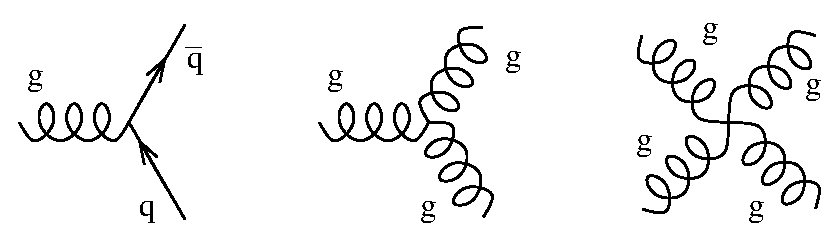
\includegraphics[width=\linewidth]{../diagram_qcd}
\end{minipage}

\vspace{0.5 cm}
\begin{itemizer}{0.5 cm}

  \item At low energies, coupling $\alpha_s$ is $\mathcal{O}(1)$,
  perturbation theory breaks down, and problems are notoriously
  difficult to solve

  \item But, formally, it's a simple theory

    \begin{itemizer}{0.5 cm}

      \item Highly symmetric

      \item 1 tunable parameter $+$ quark masses

    \end{itemizer}

  \item Electroweak force is also described by a model, but it is less satisfying:

    \begin{itemizer}{0.5 cm}

      \item CP symmetry broken (only a little bit!)

      \item No obvious pattern in flavor-changing transitions; in general, a matrix:

\[ \LARGE \hspace{3 cm} P(q_1 \to q_2) \propto \left| q_2 \cdot \left(\begin{array}{c c c} V_{ud} & V_{us} & V_{ub} \\ V_{cd} & V_{cs} & V_{cb} \\ V_{td} & V_{ts} & V_{tb} \end{array} \right) \cdot q_1 \right|^2 \hspace{2 cm} \mbox{\Huge known as CKM} \]

    \end{itemizer}

\end{itemizer}

\end{slide}

\begin{slide}

\begin{itemizer}{1 cm}

  \item Electroweak physics seems to point to something beyond itself,
  which makes it very exciting

  \item Studies have focused on pinning down the exact values of the
  CKM matrix elements, as departures from unitarity would be sure
  evidence of new physics

  \item Doing so has reminded us that QCD plays a role, one which is
  often not {\it quantitatively} understood

  \item To understand flavor physics, we need to understand color
  physics better

\end{itemizer}

\vspace{1 cm}

\end{slide}

\begin{slide}

\begin{center}
  
\includegraphics[width=5 cm]{title_outline}
\end{center}

\vspace{1 cm}

\begin{enumerate}\setlength{\itemsep}{2 cm}

  \item Follow an example of a CKM matrix element that is strictly
  limited by our ability to compute QCD

  \item Introduce Lattice QCD as a tool which can help to compute the
  necessary parameter
  
  \item Describe two CLEO experiments which test the calculation
  closely: each will be measuring the same process, substituting one
  quark for another

\end{enumerate}

\end{slide}

\begin{slide}[QCD is needed to understand electroweak physics]
  
\vfill

\begin{center}
  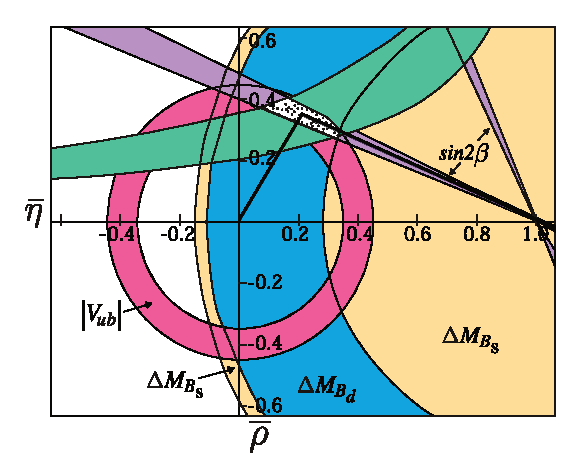
\includegraphics[width=0.55\linewidth]{../ckm04}
\end{center}

\begin{itemizer}{0.5 cm}

  \item Some of the largest uncertainties are theory uncertainties

  \item B mixing (blue) $= (known) \times ({f_B}^2 B_B) \times |V_{td}|^2$ = 0.510 $\pm$ 0.005 ps\inv\

  \item 1\% measurement!

  \item The band is $\sim$20\% because QCD factors ${f_B}^2 B_B$ are uncertain

\end{itemizer}

\end{slide}

\begin{slide}[What is this factor?]

\begin{itemizer}{1.5 cm}

  \item \begin{minipage}{0.5\linewidth} B mixing ``box diagram'' \end{minipage} \hfill \begin{minipage}{12 cm} 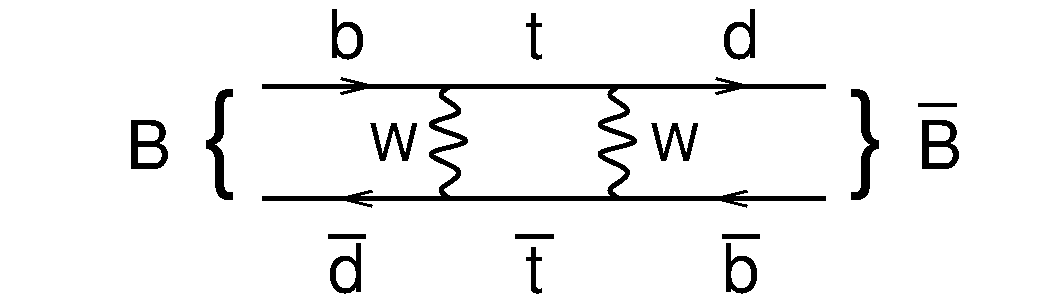
\includegraphics[width=\linewidth]{diagram_Bmix_box} \end{minipage}

  \item \begin{minipage}{0.5\linewidth} More realistic space-time diagram \end{minipage} \hfill \begin{minipage}{12 cm} 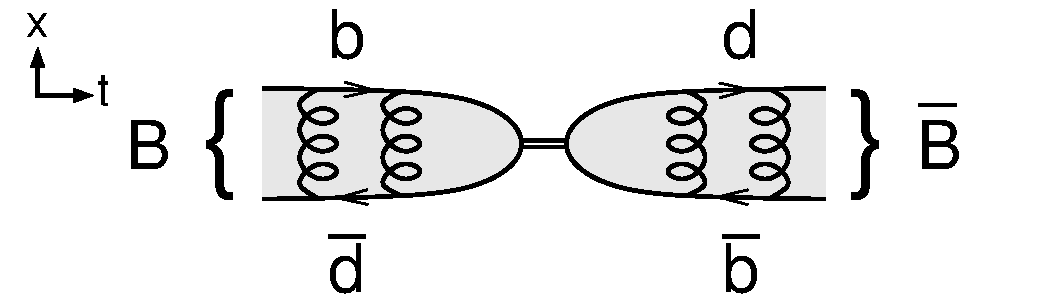
\includegraphics[width=\linewidth]{diagram_Bmix} \end{minipage}

  \item $W$ is very short-range; $\bar{d}$ is in a diffuse cloud around $b$ quark

  \item QCD interaction strength is a bottleneck for B mixing

\end{itemizer}

\end{slide}

\begin{slide}[Can $f_B$ be measured experimentally?]

\begin{itemizer}{1.5 cm}

  \item \begin{minipage}{0.5\linewidth} Leptonic mode: $B^- \to \ell^- \bar{\nu}$ \end{minipage} \hfill \begin{minipage}{12 cm} 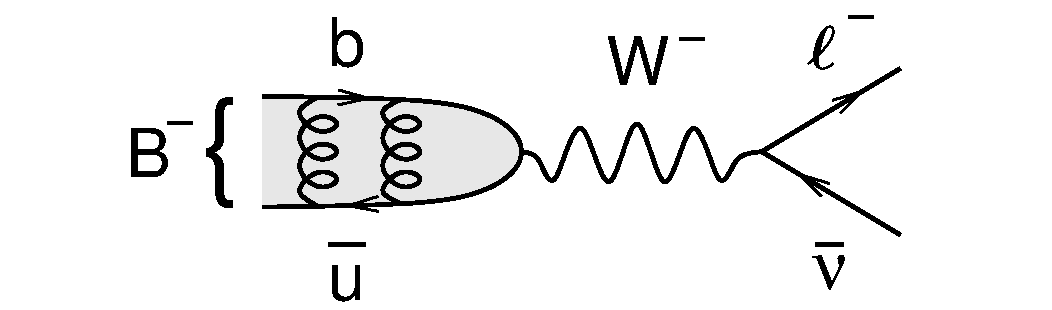
\includegraphics[width=\linewidth]{diagram_Btolnu} \end{minipage}

  \item $\displaystyle \Gamma(B^- \to \ell^- \bar{\nu}) = \frac{{G_F}^2}{8\pi} \ \underbrace{\mathheight |V_{ub}|^2 \mathheight}_{\mbox{small}} \ \underbrace{\mathheight {m_l}^2 M_B \left(1 - \frac{{m_l}^2}{{M_B}^2} \right)^2 \mathheight}_{\mbox{small}} \ {f_B}^2$

    \vspace{0.5 cm}
  \item ${\cal B}(B^- \to \tau^- \bar{\nu}) <$ $\mathsf{2.6 \times 10^{-4}}$ at 90\% C.L. (BaBar)

\end{itemizer}

\end{slide}

\begin{slide}[Can $f_B$ be calculated theoretically?]

\begin{itemizer}{1 cm}

  \item Deriving the QCD potential/wavefunctions is a non-perturbative problem

  \item Most promising technique: Lattice QCD (LQCD)

\end{itemizer}

\vspace{1 cm}
\begin{minipage}{0.5\linewidth}
  \begin{itemizer}{1 cm}
    \item Represent space-time as a 4-D grid of quark and gluon field values

    \item Evaluate Feynman path integral

    \item Number of {\it dimensions} in that \mbox{integral} scales
    with number of \mbox{pixels}

  \end{itemizer}
\end{minipage} \hfill \begin{minipage}{0.45\linewidth}
  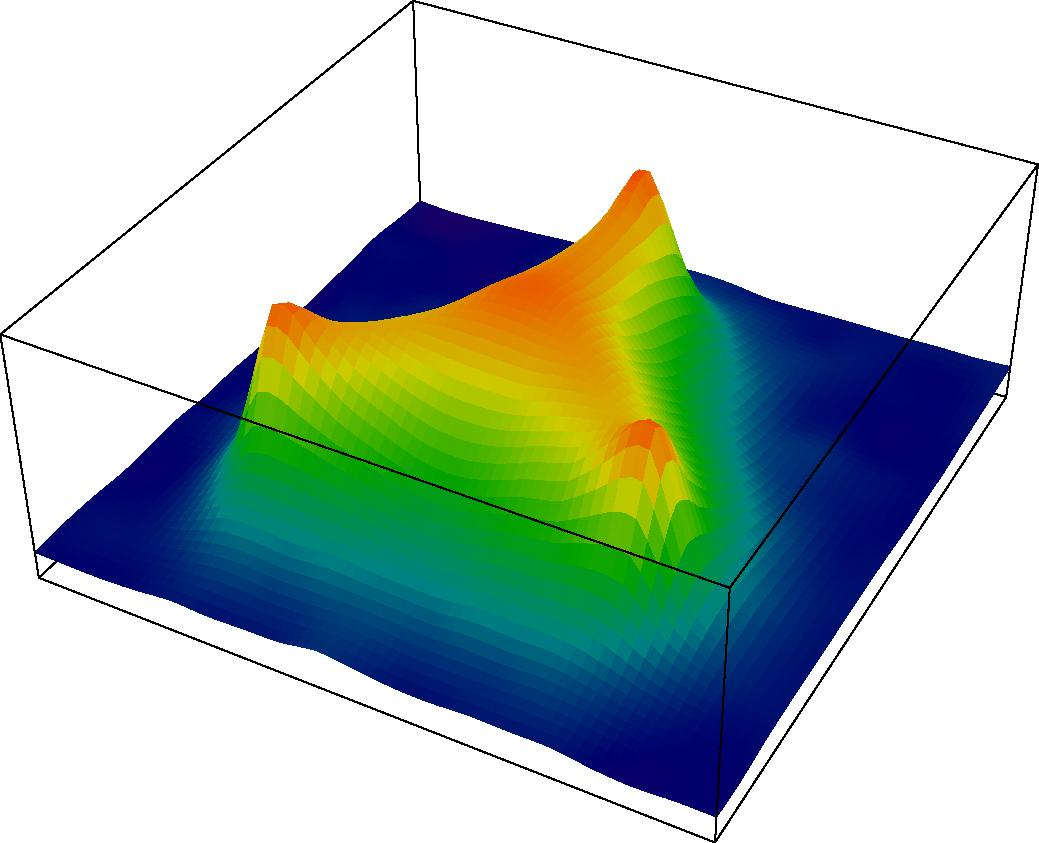
\includegraphics[width=\linewidth]{../qcd_proton}
\end{minipage}

\vspace{1 cm}
\begin{itemizer}{1 cm}

  \item Very computationally intensive: many problems are intractable

\end{itemizer}

\end{slide}

\begin{slide}[Approximation to simplify calculation]

\begin{itemizer}{2 cm}

  \item \begin{minipage}{0.6\linewidth} Try ignoring light quark loops (``quenched'') \end{minipage} \hfill \begin{minipage}{7 cm} 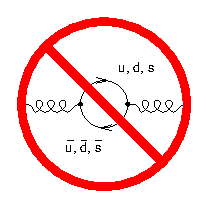
\includegraphics[width=\linewidth]{quenched} \end{minipage}

  \item Until c.\ 2000, this was necessary for physical calculations

  \item Introduces large (10--20\%) uncertainties that are difficult to assess

\end{itemizer}

\end{slide}

\begin{slide}[Precision LQCD]

\begin{itemize}

  \item Improved algorithms allow ``unquenched,'' realistic
    calculations with few percent uncertainties

\end{itemize}

\vspace{0.5 cm}
\begin{center}
  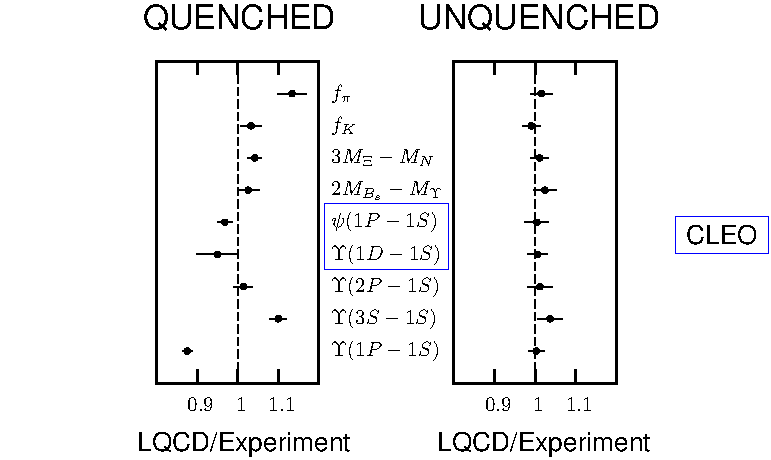
\includegraphics[width=0.9\linewidth, trim=0 0.5cm 0 0.4cm]{lqcd_success2}
\end{center}

\vspace{0.5 cm}
\begin{itemize}

  \item Update: $\Omega^-$ and $B_c$ masses work also

\end{itemize}

\end{slide}

\begin{slide}[CLEO contributions]

\vspace{-1.5 cm}
\begin{minipage}{0.6\linewidth}
  \begin{itemize}

    \item ``$\psi(1P-1S)$'': observation of $h_c$ with mass
    3524.4 $\pm$ 0.6 $\pm$ 0.4 MeV (2005)

  \end{itemize}
\end{minipage} \hfill \begin{minipage}{0.38\linewidth}
  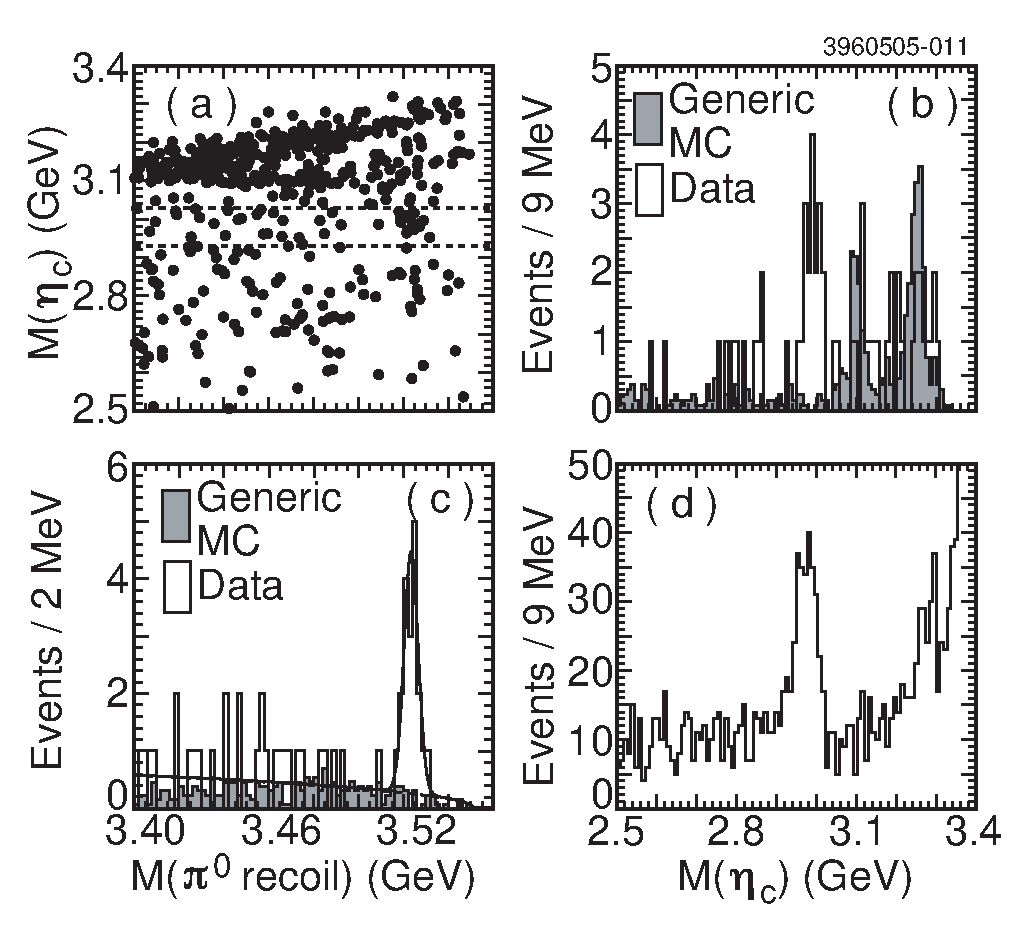
\includegraphics[width=\linewidth, trim=0 0 8.5cm 7cm, clip=true]{discovery_hc}
\end{minipage}

\begin{minipage}{0.6\linewidth}
  \begin{itemize}

    \item ``$\Upsilon(1D-1S)$'': discovery of $\Upsilon(1D)$ with mass
    10161.1 $\pm$ 0.6 $\pm$ 1.6 MeV (2004)

  \end{itemize}
\end{minipage} \hfill \begin{minipage}{0.38\linewidth}
  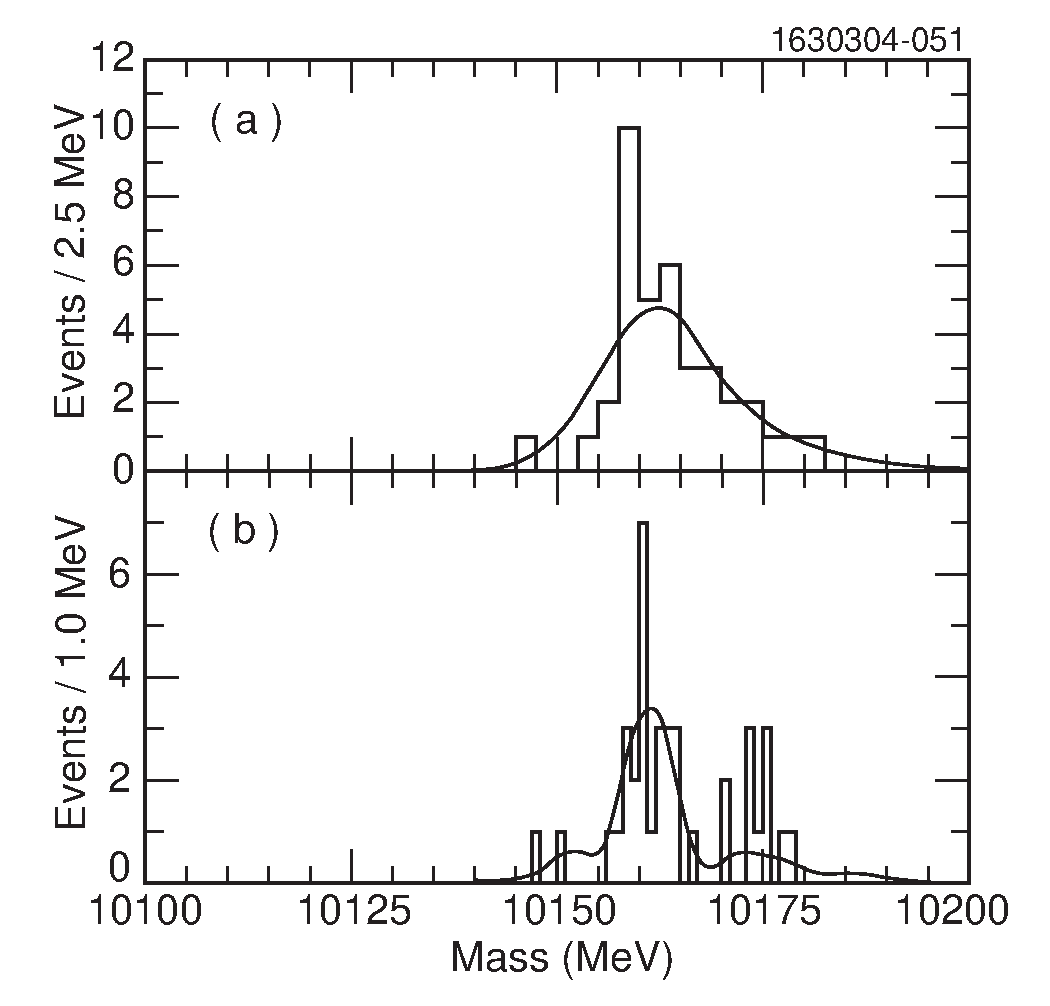
\includegraphics[width=\linewidth]{discovery_1d}
\end{minipage}

\vspace{-0.5 cm}

\end{slide}

\begin{slide}[How to check $f_B$ calculation: swap quarks]

\begin{itemizer}{2 cm}

  \item \begin{minipage}{0.22\linewidth} $f_B$ \end{minipage} \hfill \begin{minipage}{11 cm} 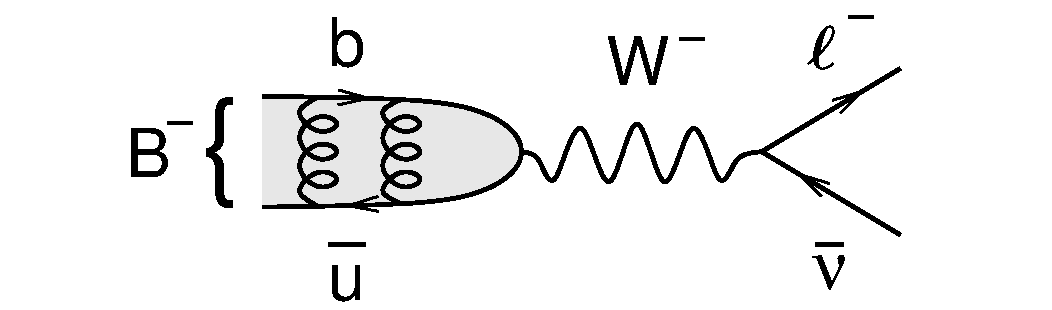
\includegraphics[width=\linewidth]{diagram_Btolnu} \end{minipage} \hfill \begin{minipage}{0.3\linewidth} \begin{center} LQCD only \end{center} \end{minipage}

  \item \begin{minipage}{0.22\linewidth} $\Gamma(\Upsilon \to e^+e^-)$ \end{minipage} \hfill \begin{minipage}{11 cm} 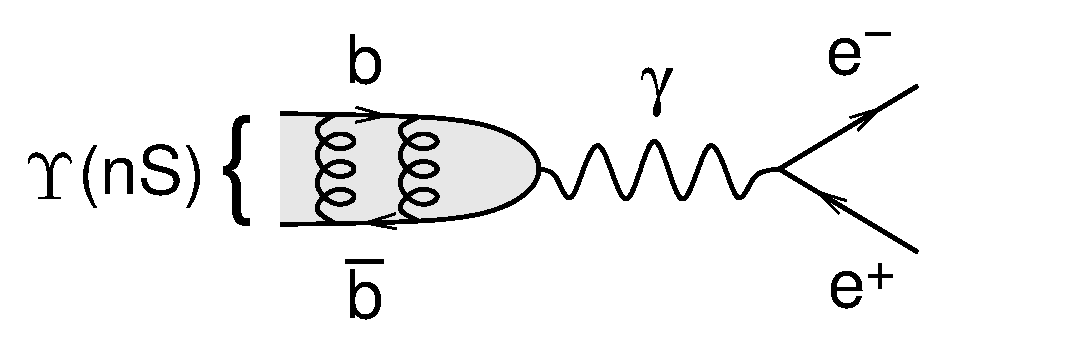
\includegraphics[width=\linewidth]{diagram_GeeU} \end{minipage} \hfill \begin{minipage}{0.3\linewidth} \begin{center} LQCD vs CLEO-III \end{center} \end{minipage}

  \item \begin{minipage}{0.22\linewidth} $f_D$ \end{minipage} \hfill \begin{minipage}{11 cm} 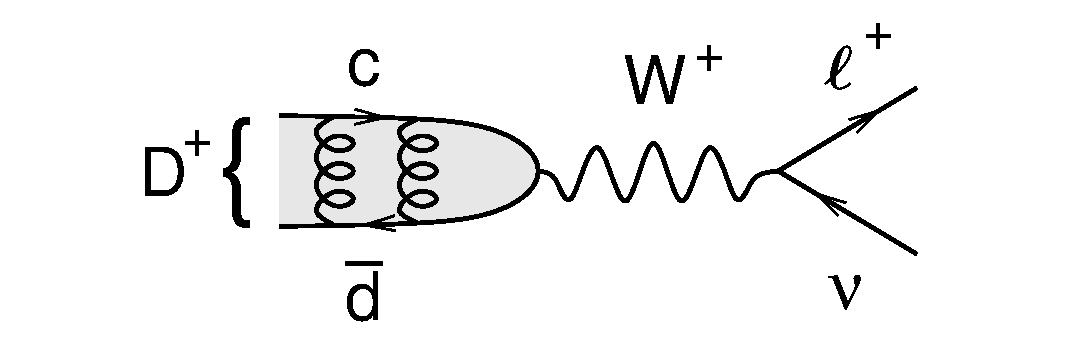
\includegraphics[width=\linewidth]{diagram_Dtolnu} \end{minipage} \hfill \begin{minipage}{0.3\linewidth} \begin{center} LQCD vs CLEO-c \end{center} \end{minipage}

\end{itemizer}

\vfill

\end{slide}

\begin{slide}

\vfill
\begin{center}
  \fbox{
\includegraphics[height=1.5 cm]{title_GeeU}}
\end{center}

\vfill
\begin{itemizer}{1 cm}

  \item Three results, 1.5--3\% precision

  \item Outline will be at the top of the screen

\end{itemizer}

\vfill

\end{slide}

\begin{slidemap1}[{\color{blue} technique} & backgrounds & efficiency & luminosity & stability & fits & results & theory]

\begin{itemizer}{0.5 cm}

  \item By definition, $\Gamma_{ee}(\Upsilon)$ is the decay rate of
  $\Upsilon$ to $e^+e^-$

\[ \Gamma_{ee} = \Gamma \times \mathcal{B}_{ee} \mbox{ where $\Gamma$ is the resonance width} \]

  \item It may seem that a measurement would consist of counting $e^+e^-$, but

    \vspace{0.2 cm}
    \begin{itemizer}{0.4 cm}
      \item this measures $\mathcal{B}_{ee}$, which is a step removed
      from $\Gamma_{ee}$

      \item $\Gamma$ can't be measured directly
    \end{itemizer}

  \item Alternative method: consider time-reversed process

  \begin{center}
    \begin{tabular}{p{10 cm} c p{10 cm}}
      \begin{minipage}{\linewidth} \begin{center}
  	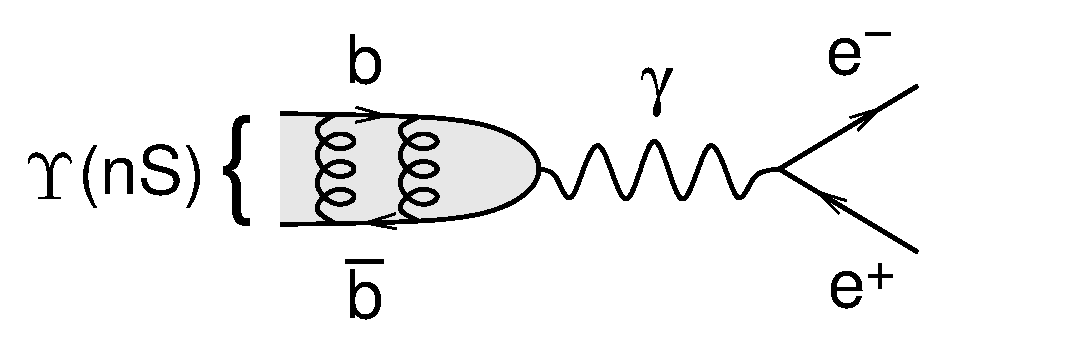
\includegraphics[width=10 cm]{diagram_GeeU} \mbox{\hspace{-1 cm}}
      \end{center} \end{minipage} & \mbox{\hspace{0.2 cm}} $\to$ \mbox{\hspace{0.2 cm}} &
      \begin{minipage}{\linewidth} \begin{center}
  	\mbox{\hspace{-1 cm}} 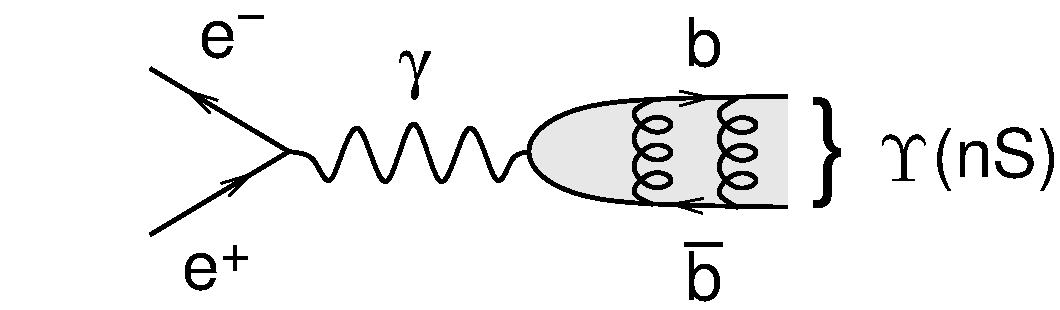
\includegraphics[width=10 cm]{diagram_GeeU-reversed}
      \end{center} \end{minipage}
    \end{tabular}
  \end{center}

  \item Measure $\Upsilon$ {\it production} from $e^+e^-$ beams

\[ \Gamma_{ee} = \frac{{M_\Upsilon}^2}{6 \pi^2} \int \sigma(e^+e^- \to \Upsilon) \, dE \]

\end{itemizer}

\end{slidemap1}

\begin{slidemap1}[{\color{blue} technique} & backgrounds & efficiency & luminosity & stability & fits & results & theory]

\begin{itemize}

  \item Scan $\Upsilon$ resonance to perform $dE$ integration

  \item Cross-section versus beam energy $\to$ integrated cross-section $\to$ $\Gamma_{ee}$

\end{itemize}

\vspace{0.5 cm}
\begin{center}
  \begin{tabular}{p{0.45\linewidth} c p{0.35\linewidth}}
    \begin{minipage}{\linewidth}
      \begin{center}
	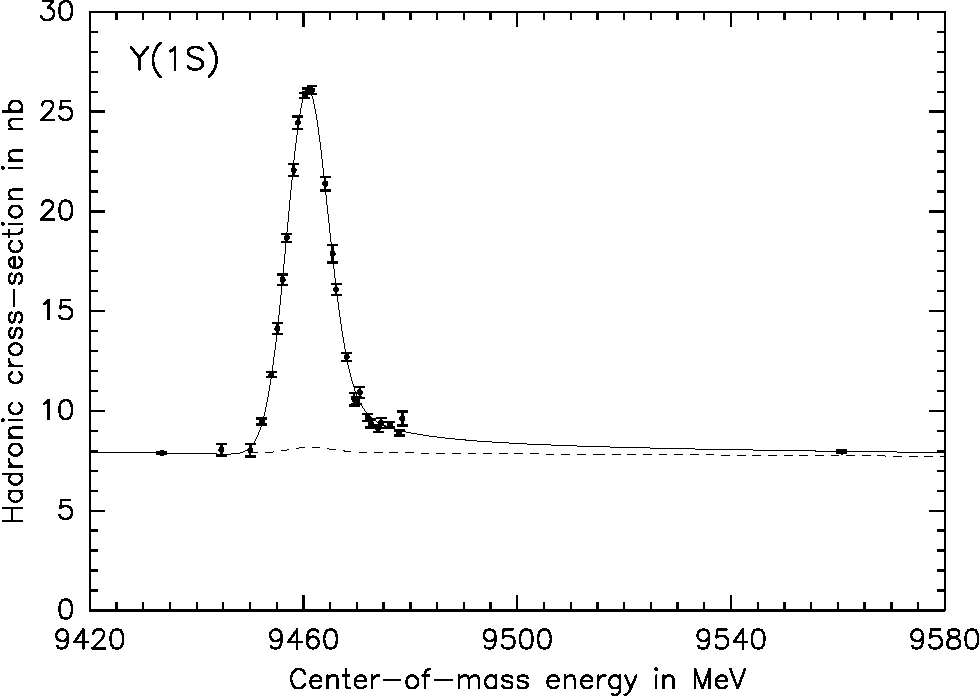
\includegraphics[width=\linewidth]{individual07_noinset_1s}

	\vspace{0.25 cm}
	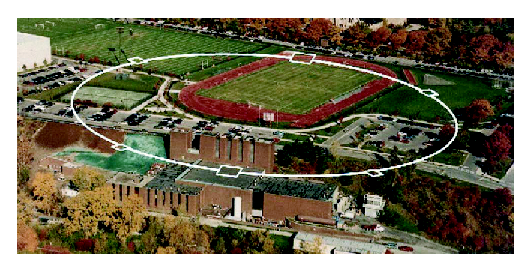
\includegraphics[width=0.7\linewidth]{aerial2}
      \end{center}
    \end{minipage} & \mbox{\hspace{0.25 cm}} &
    \begin{minipage}{\linewidth}
      \begin{itemizer}{1 cm}

	\item Dedicated scans

	\item $\displaystyle \int$Luminosity in fb\inv

	  \begin{center}
	    \renewcommand{\arraystretch}{1.25}
	    \begin{tabular}{c c c}
	      & scan & off-res \\\hline
	      1S & 0.27 & 0.19 \\
	      2S & 0.08 & 0.41 \\
	      3S & 0.22 & 0.14 \\
	    \end{tabular}
	  \end{center}

	\item Nov 2001 -- Aug 2002

      \end{itemizer}
    \end{minipage} \\
    \begin{minipage}{\linewidth} \begin{center} \LARGE Cornell Electron Storage Ring \end{center} \end{minipage} & &
  \end{tabular}
\end{center}

\end{slidemap1}

\begin{slidemap1}[{\color{blue} technique} & backgrounds & efficiency & luminosity & stability & fits & results & theory]

\vspace{0.3 cm}

\begin{center}
  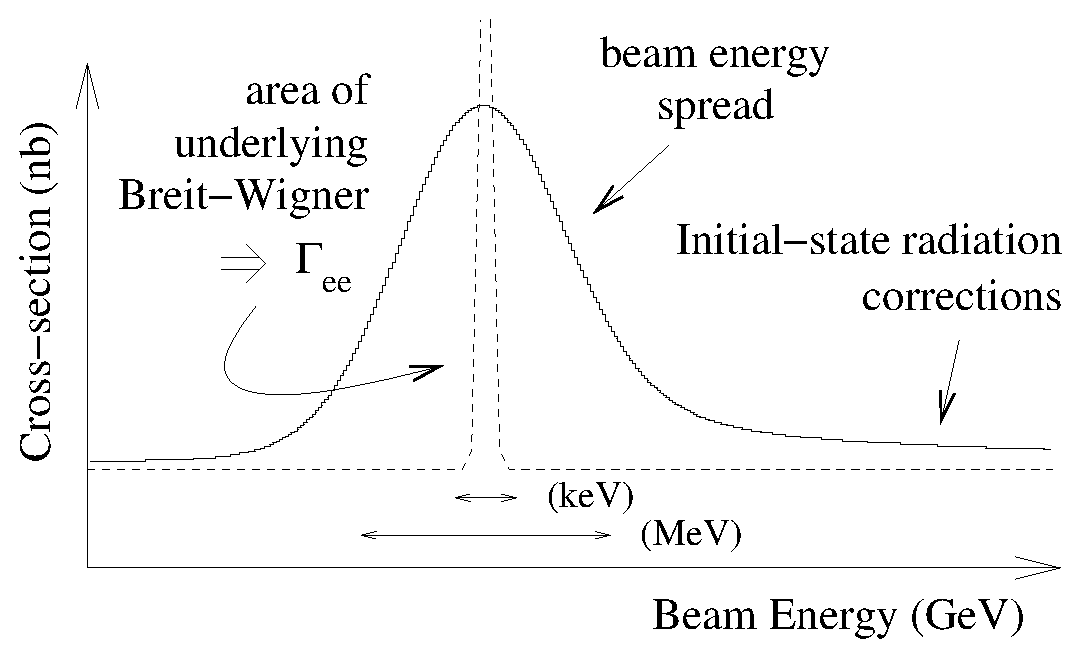
\includegraphics[width=0.55\linewidth]{../cartoon}
\end{center}

\begin{itemizer}{0.6 cm}

  \item Most background processes scale as $1/s$

  \item Breit-Wigner (BW) lineshape is convoluted with beam energy
  spread: \\ does not affect {\it area} (= $\Gamma_{ee}$)

  \item Also convoluted with ISR tail ($e^+e^- \to \gamma \Upsilon$)
  which diverges

  \item {\boldmath Fit to BW $\otimes$ Gauss $\otimes$ ISR, quote BW area}

\end{itemizer}

\end{slidemap1}

\begin{slidemap1}[{\color{blue} technique} & backgrounds & efficiency & luminosity & stability & fits & results & theory]

\vspace{0.3 cm}

\begin{itemizer}{0.3 cm}

  \item Majority of $\Upsilon$ events are hadronic; well-measured fraction are $\ell^+\ell^-$

  \item Design event selection for $\Upsilon \to$ hadrons

\end{itemizer}

\vfill

\begin{center}
  \begin{tabular}{p{0.6\linewidth} p{0.3\linewidth}}
    \begin{minipage}{\linewidth}
      \begin{center}
	\LARGE Solid = data, dashed = scaled Monte Carlo, log scale

	\vspace{0.5 cm}
	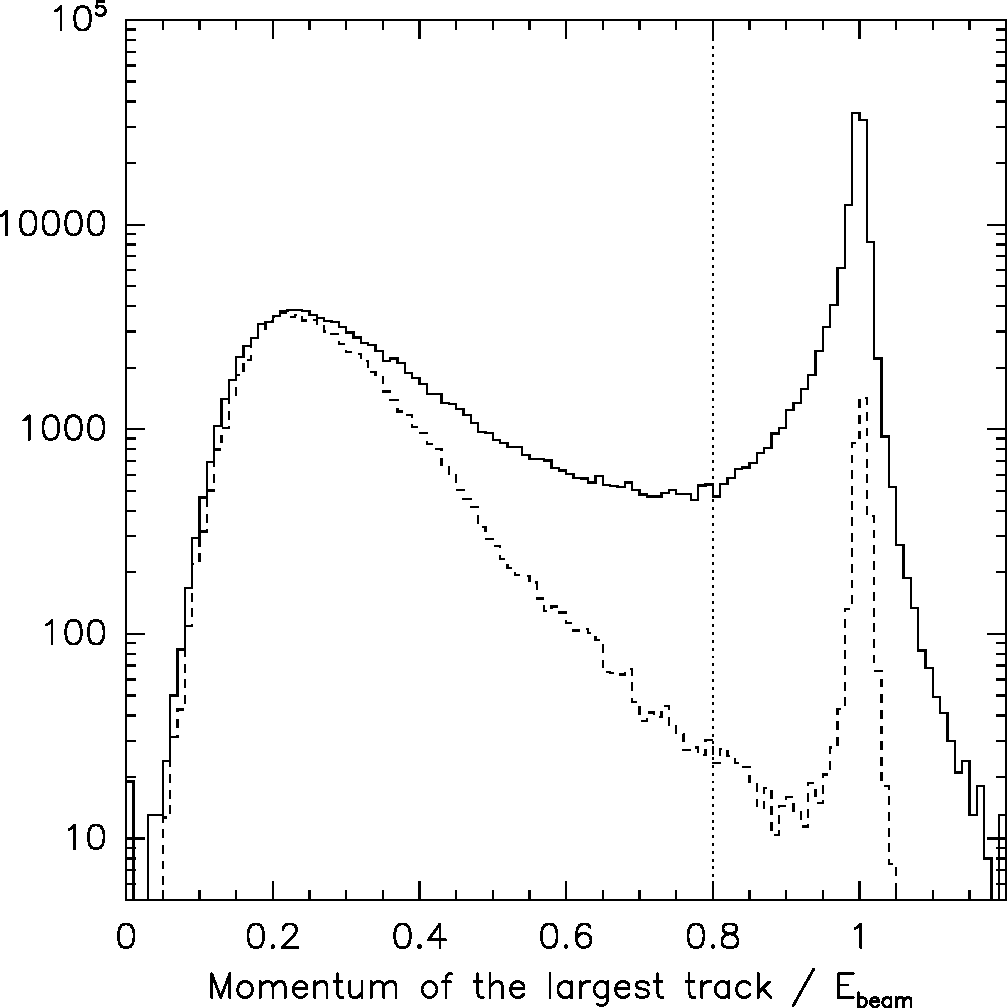
\includegraphics[width=0.8\linewidth]{cuts_p1} \mbox{\hspace{1 cm}}
      \end{center}
    \end{minipage} & 
    \begin{minipage}{\linewidth}
      Cut out

      \vspace{0.5 cm}
      \begin{enumerate}\setlength{\itemsep}{1 cm}

	\item \textcolor{blue}{Bhabhas}

	\item \textcolor{white}{Two-photon fusion}

	\item \textcolor{white}{Cosmic rays}

	\item \textcolor{white}{Beam-gas}

      \end{enumerate}
    \end{minipage}
  \end{tabular}
\end{center}

\end{slidemap1}

\begin{slidemap1}[{\color{blue} technique} & backgrounds & efficiency & luminosity & stability & fits & results & theory]

\vspace{0.3 cm}

\begin{itemizer}{0.3 cm}

  \item Majority of $\Upsilon$ events are hadronic; well-measured fraction are $\ell^+\ell^-$

  \item Design event selection for $\Upsilon \to$ hadrons

\end{itemizer}

\vfill

\begin{center}
  \begin{tabular}{p{0.6\linewidth} p{0.3\linewidth}}
    \begin{minipage}{\linewidth}
      \begin{center}
	\LARGE Solid = data, dashed = scaled Monte Carlo, log scale

	\vspace{0.5 cm}
	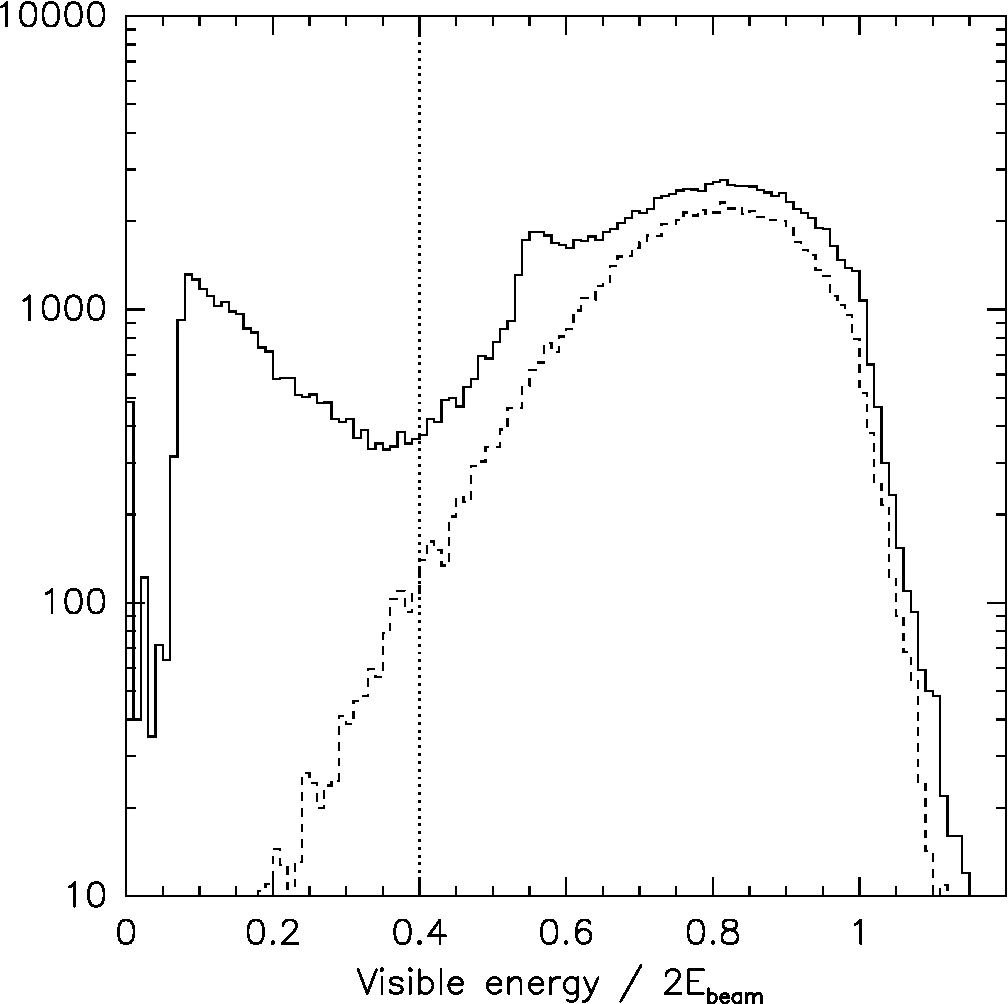
\includegraphics[width=0.8\linewidth]{cuts_visen} \mbox{\hspace{1 cm}}
      \end{center}
    \end{minipage} & 
    \begin{minipage}{\linewidth}
      Cut out

      \vspace{0.5 cm}
      \begin{enumerate}\setlength{\itemsep}{1 cm}

	\item \textcolor{black}{Bhabhas}

	\item \textcolor{blue}{Two-photon fusion}

	\item \textcolor{white}{Cosmic rays}

	\item \textcolor{white}{Beam-gas}

      \end{enumerate}
    \end{minipage}
  \end{tabular}
\end{center}

\end{slidemap1}

\begin{slidemap1}[{\color{blue} technique} & backgrounds & efficiency & luminosity & stability & fits & results & theory]

\vspace{0.3 cm}

\begin{itemizer}{0.3 cm}

  \item Majority of $\Upsilon$ events are hadronic; well-measured fraction are $\ell^+\ell^-$

  \item Design event selection for $\Upsilon \to$ hadrons

\end{itemizer}

\vfill

\begin{center}
  \begin{tabular}{p{0.6\linewidth} p{0.3\linewidth}}
    \begin{minipage}{\linewidth}
      \begin{center}
	\LARGE Solid = data, dashed = scaled Monte Carlo, log scale

	\vspace{0.5 cm}
	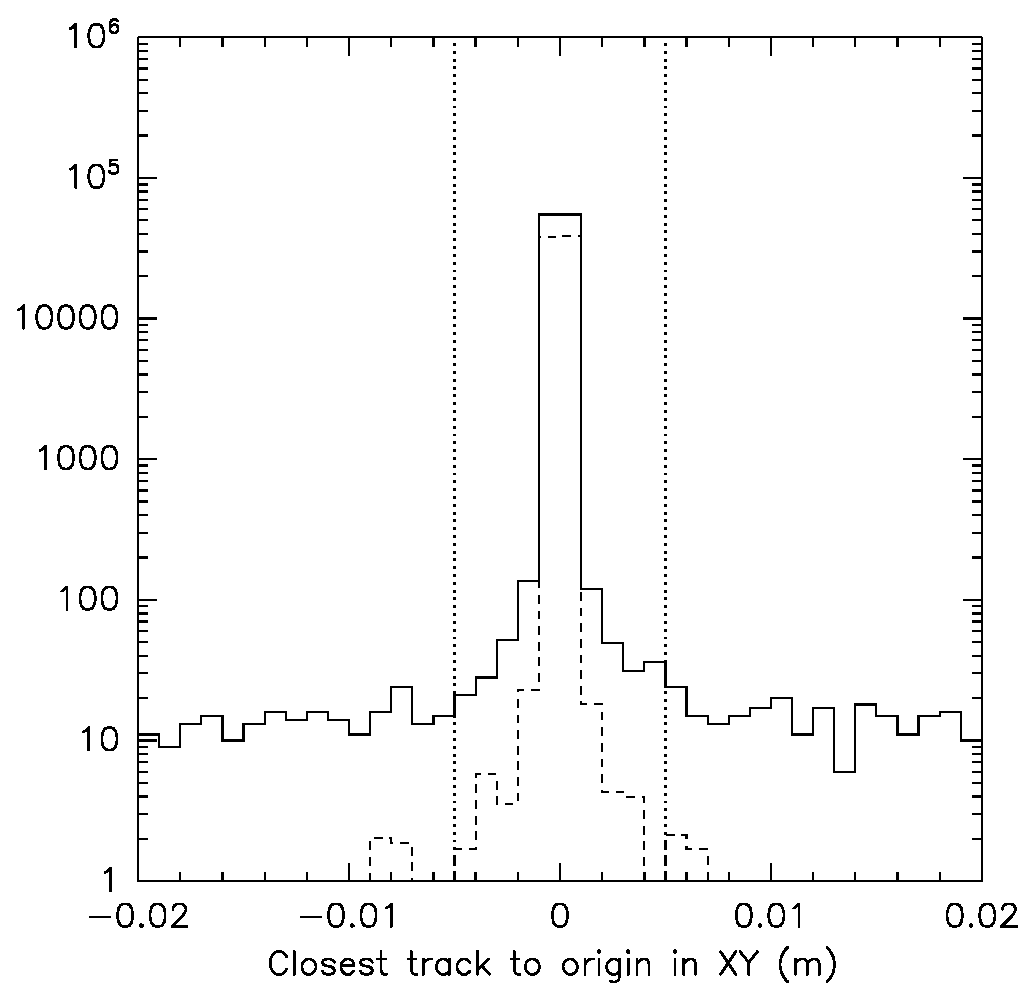
\includegraphics[width=0.8\linewidth]{cuts_d0close} \mbox{\hspace{1 cm}}
      \end{center}
    \end{minipage} & 
    \begin{minipage}{\linewidth}
      Cut out

      \vspace{0.5 cm}
      \begin{enumerate}\setlength{\itemsep}{1 cm}

	\item \textcolor{black}{Bhabhas}

	\item \textcolor{black}{Two-photon fusion}

	\item \textcolor{blue}{Cosmic rays}

	\item \textcolor{white}{Beam-gas}

      \end{enumerate}
    \end{minipage}
  \end{tabular}
\end{center}

\end{slidemap1}

\begin{slidemap1}[{\color{blue} technique} & backgrounds & efficiency & luminosity & stability & fits & results & theory]

\vspace{0.3 cm}

\begin{itemizer}{0.3 cm}

  \item Majority of $\Upsilon$ events are hadronic; well-measured fraction are $\ell^+\ell^-$

  \item Design event selection for $\Upsilon \to$ hadrons

\end{itemizer}

\vfill

\begin{center}
  \begin{tabular}{p{0.6\linewidth} p{0.3\linewidth}}
    \begin{minipage}{\linewidth}
      \begin{center}
	\LARGE Solid = data, dashed = scaled Monte Carlo, log scale

	\vspace{0.5 cm}
	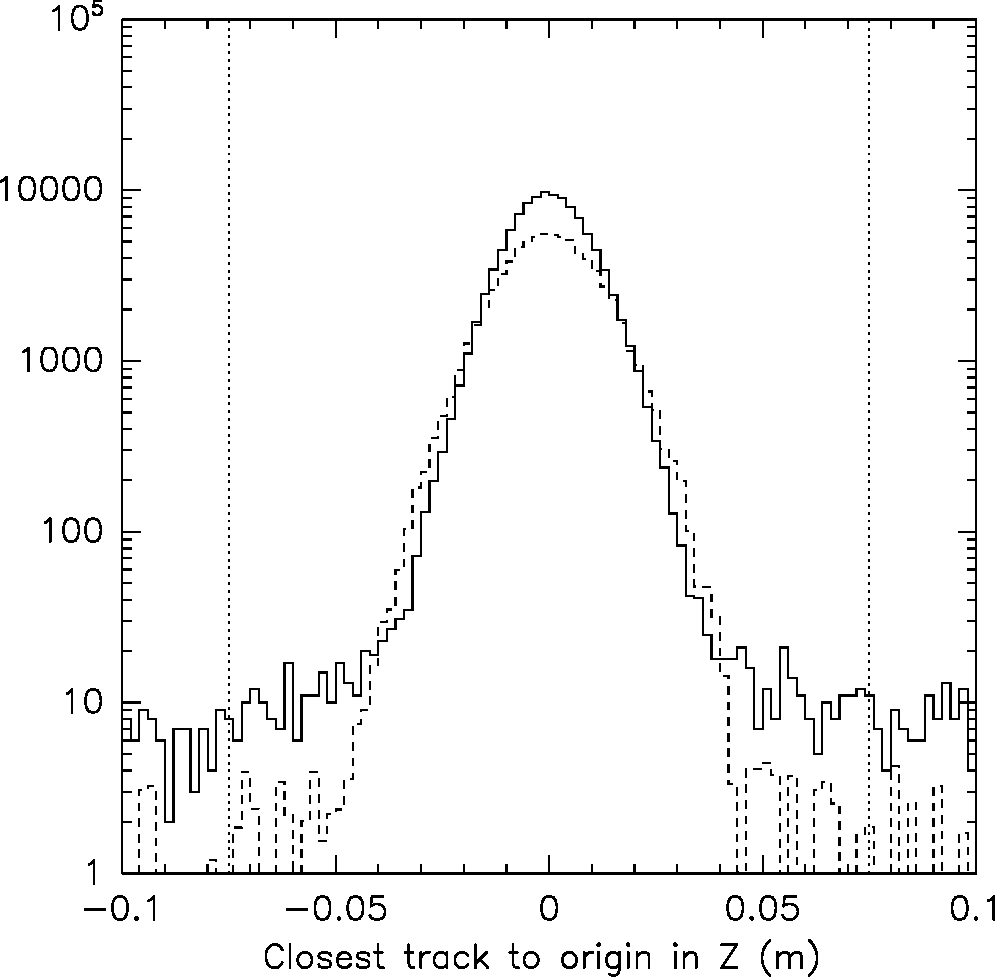
\includegraphics[width=0.8\linewidth]{cuts_anyz} \mbox{\hspace{1 cm}}
      \end{center}
    \end{minipage} & 
    \begin{minipage}{\linewidth}
      Cut out

      \vspace{0.5 cm}
      \begin{enumerate}\setlength{\itemsep}{1 cm}

	\item \textcolor{black}{Bhabhas}

	\item \textcolor{black}{Two-photon fusion}

	\item \textcolor{black}{Cosmic rays}

	\item \textcolor{blue}{Beam-gas}

      \end{enumerate}
    \end{minipage}
  \end{tabular}
\end{center}

\end{slidemap1}

\begin{slidemap1}[technique & {\color{blue} backgrounds} & efficiency & luminosity & stability & fits & results & theory]

\begin{center}
%   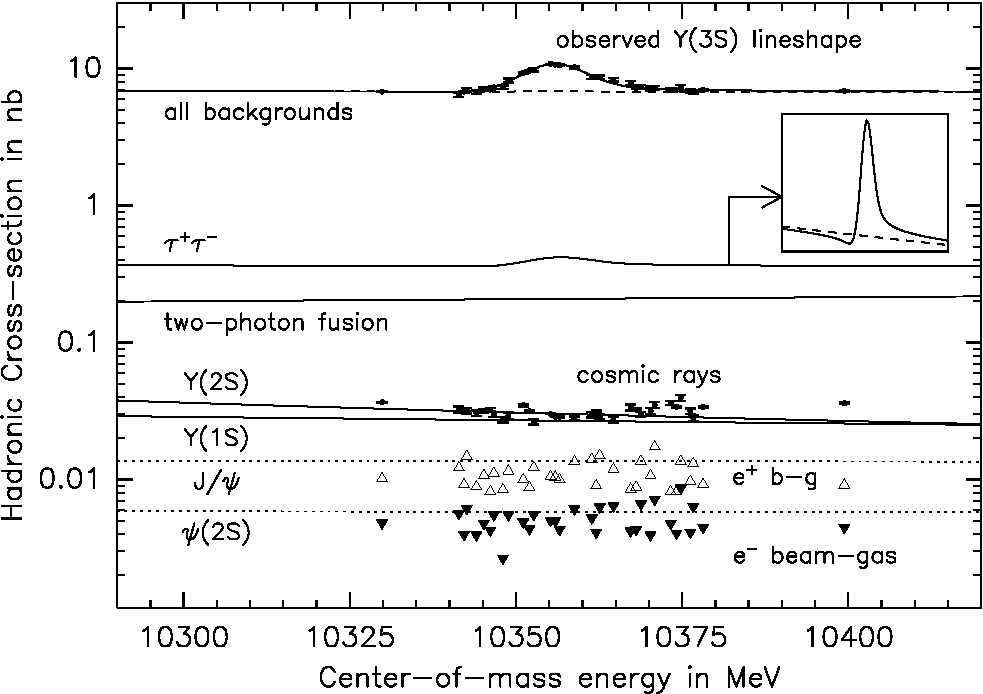
\includegraphics[width=0.9\linewidth, trim=0.5cm 2cm 0.5cm 2cm]{../jed_backgrounds}
  \includegraphics[width=0.9\linewidth, trim=0.5cm 2cm 0.5cm 2cm]{/home/mccann/antithesis/plots/panic05/prettied_notau_backgrounds_6}
\end{center}

\end{slidemap1}

\begin{slidemap1}[technique & {\color{blue} backgrounds} & efficiency & luminosity & stability & fits & results & theory]

\begin{center}
  \begin{tabular}{p{0.65\linewidth} c p{0.3\linewidth}}
    \begin{minipage}{\linewidth}
      \begin{center}
	\LARGE Histogram is side-band data, points are control sample, log-$x$ axis

	\vspace{0.25 cm}
	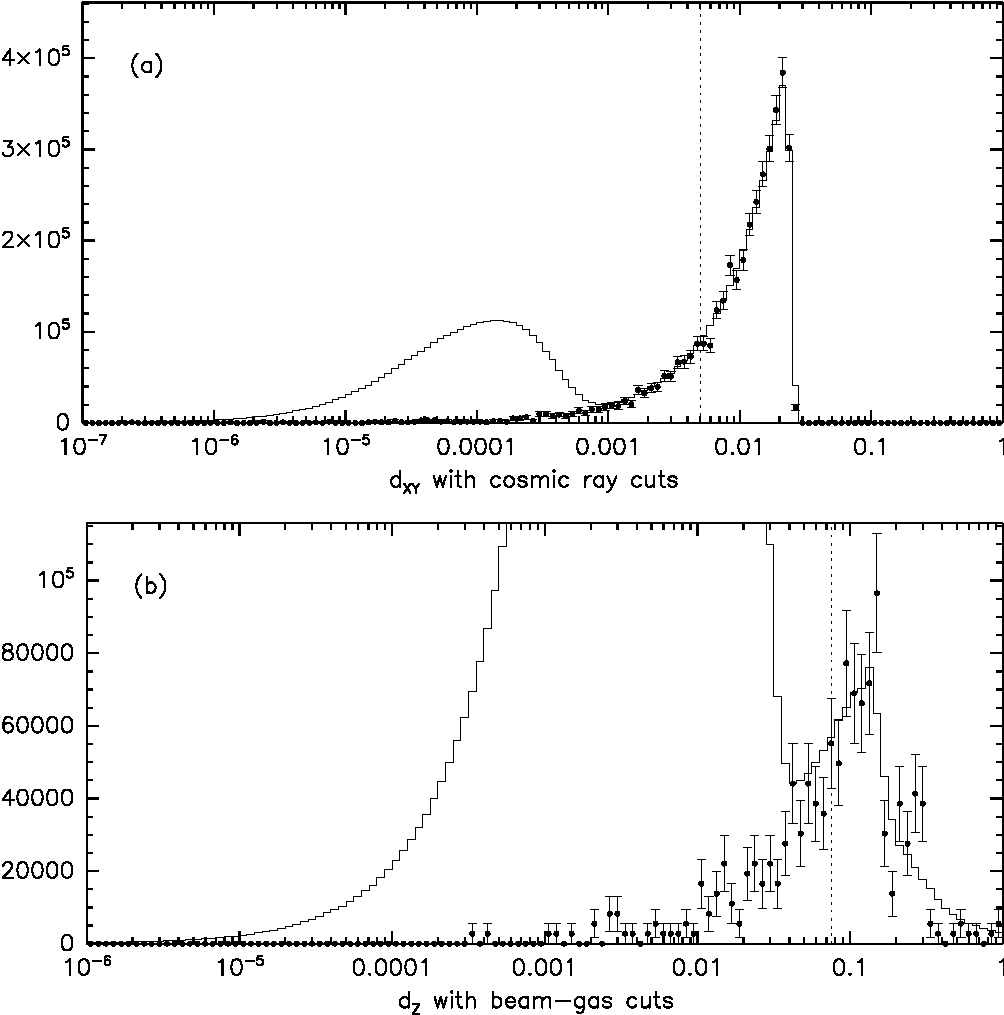
\includegraphics[width=\linewidth]{../datasets_database_dxydzcuts}
      \end{center}
    \end{minipage} & &
    \begin{minipage}{\linewidth}
      (a) Cosmic ray sideband: normalize with ``no-beam'' sample

      \vspace{0.5 cm}
      {\LARGE (XY distance from beamspot)}

      \vspace{4 cm}

      (b) Beam-gas sideband: normalize with ``single-beam'' sample

      \vspace{0.5 cm}
      {\LARGE (Z distance from beamspot)}

      \vspace{0.5 cm}
    \end{minipage}
  \end{tabular}
\end{center}

\end{slidemap1}

\begin{slidemap1}[technique & backgrounds & {\color{blue} efficiency} & luminosity & stability & fits & results & theory]

\begin{itemizer}{0.5 cm}

  \item How many hadronic $\Upsilon$ decays pass event selection?

  \item Model-independent method for measuring hadronic
    efficiency:

    \begin{tabular}{p{0.48\linewidth} c p{0.5\linewidth}}
      \begin{minipage}{\linewidth}
	\vspace{1 cm}
        \begin{itemizer}{0.5 cm}

          \item Select \mbox{$\Upsilon(2S) \to \pi^+ \pi^- \ \Upsilon(1S)$} based on $\pi^+ \pi^-$ only	    

	  \item Choose $\pi^+ \pi^-$ to be sufficient for all cuts, trigger

          \item Set of $\Upsilon(1S)$ events is unbiased

	    \vspace{0.5 cm}
	    Includes all decays, even if \\ undetectable


          \item \#pass/\#total = (97.8 $\pm$ 0.5)\%

        \end{itemizer}
      \end{minipage} & & \begin{minipage}{\linewidth}
	\vspace{0.5 cm}
	\includegraphics[width=\linewidth]{/home/mccann/antithesis/plots/panic05/prettied_plenary_justpipimass}

	\vspace{-0.75 cm}
      \end{minipage}
    \end{tabular}

\end{itemizer}

\vfill

\end{slidemap1}

\begin{slidemap1}[technique & backgrounds & {\color{blue} efficiency} & luminosity & stability & fits & results & theory]

\begin{itemize}

  \item Events in $\Upsilon$ peak (cut variables)

\end{itemize}

\begin{center}
  \LARGE Histogram is Monte Carlo, points are data

  \vspace{0.25 cm}
  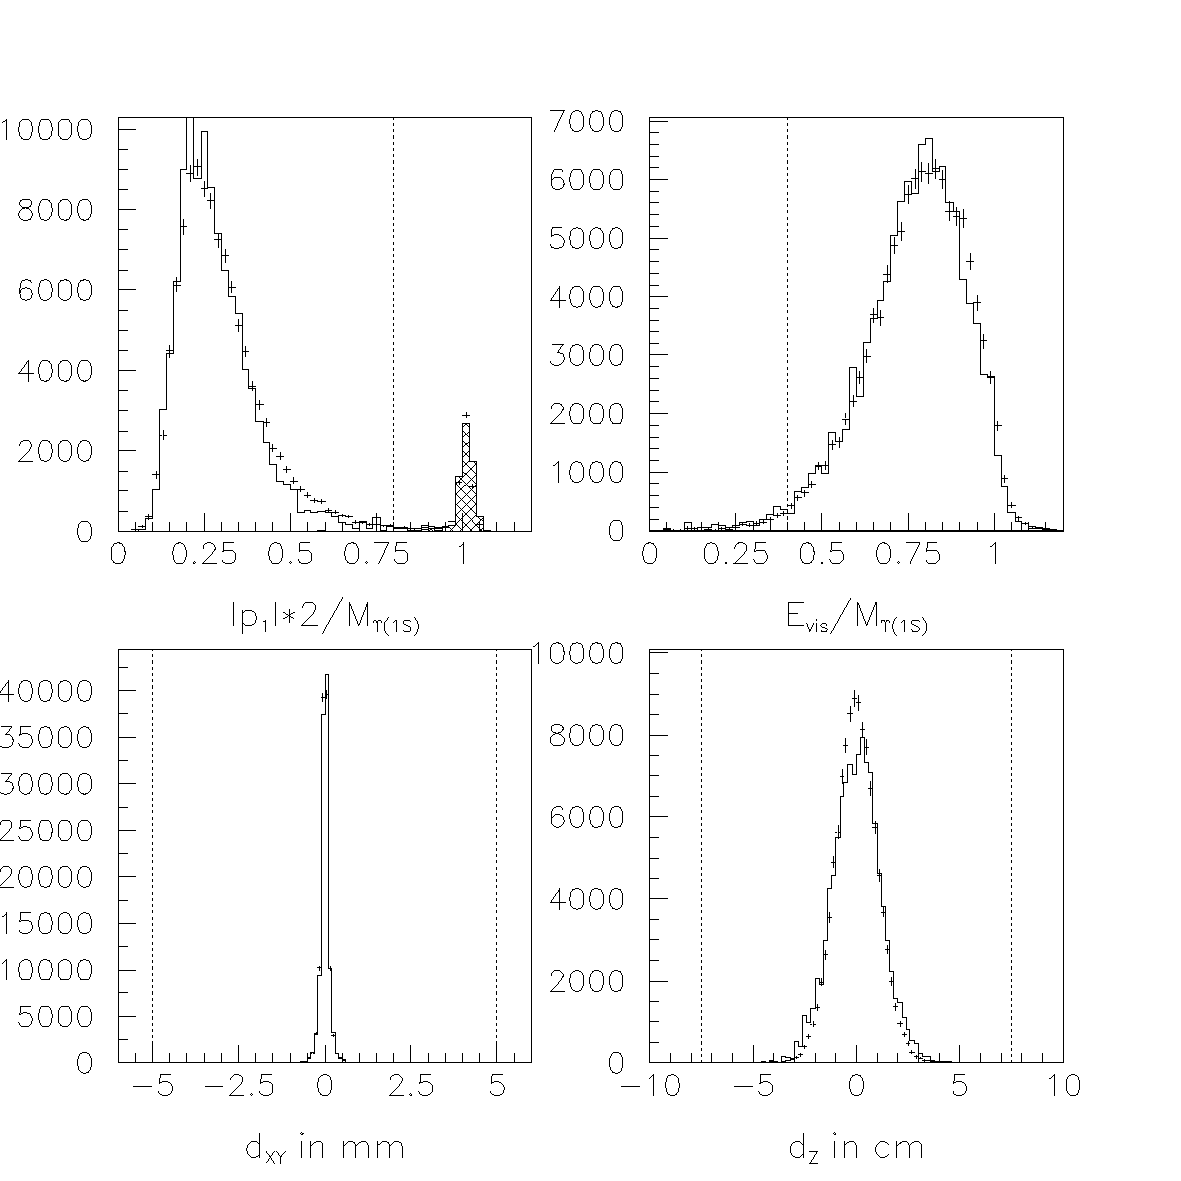
\includegraphics[width=0.6\linewidth, trim=0 0 1.5cm 2cm]{proceedings_cuts2}
\end{center}

\end{slidemap1}

\begin{slidemap1}[technique & backgrounds & {\color{blue} efficiency} & luminosity & stability & fits & results & theory]

\begin{itemizer}{0.75 cm}

  \item For $\Upsilon(2S)$, $\Upsilon(3S)$, most modes are unchanged

  \item Exception: $\textcolor{blue}{X} \textcolor{red}{e^+e^-}$ and $\textcolor{blue}{X} \textcolor{red}{\mu^+\mu^-}$, which have zero efficiency

    \hfill (track momentum cut)

\end{itemizer}

\begin{center}
  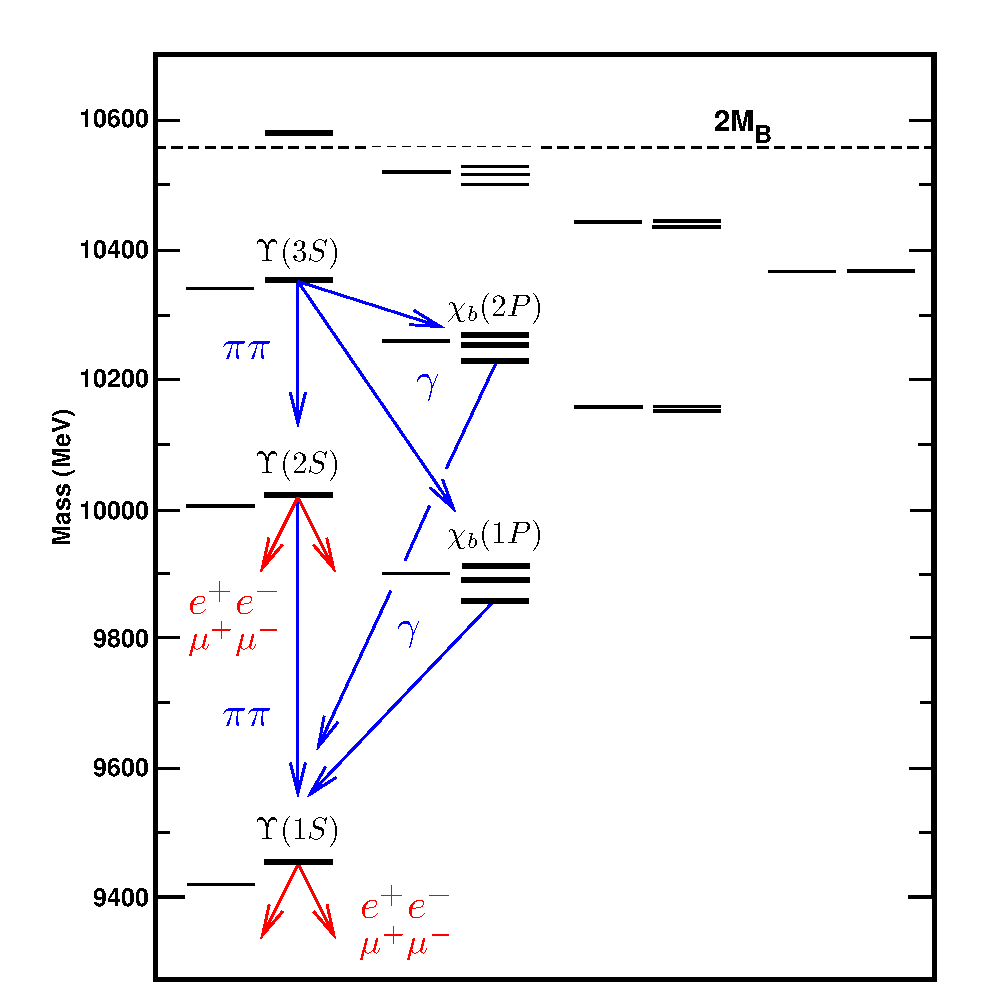
\includegraphics[width=0.5\linewidth]{ups_spectrum2}
\end{center}

\end{slidemap1}

\begin{slidemap1}[technique & backgrounds & {\color{blue} efficiency} & luminosity & stability & fits & results & theory]

\vspace{0.5 cm}
\begin{itemizer}{0.75 cm}

  \item $\Upsilon(2S)$, $\Upsilon(3S)$ efficiency is essentially 1 $-$ ${\cal B}(\textcolor{blue}{X} \textcolor{red}{\ell^+\ell^-})$

  \item Mini-analysis to determine these branching fractions in data

\end{itemizer}

\vspace{0.5 cm}
\begin{center}
  \LARGE $\textcolor{red}{\mu^+\mu^-}$ invariant mass, histogram is Monte Carlo, points are data, shaded is {\it prompt} $\mu^+\mu^-$ (no $\textcolor{blue}{X}$)

  \vspace{0.35 cm}
  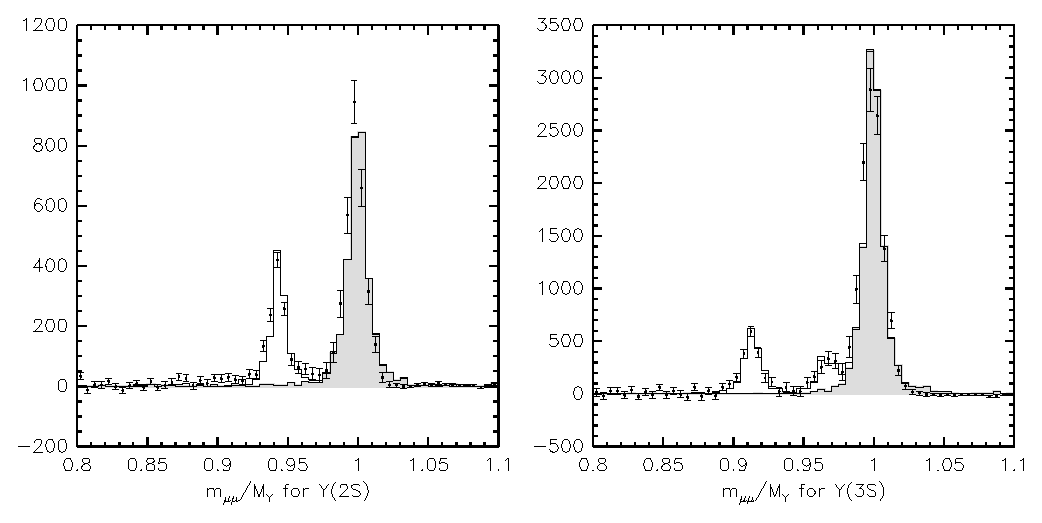
\includegraphics[width=0.8\linewidth]{../beautiful_bcasll_2}
\end{center}

\begin{itemizer}{0.75 cm}

  \item ${\cal B}(2S \to \textcolor{blue}{X} \textcolor{red}{\ell^+\ell^-})$ = (1.58 $\pm$ 0.16)\% \hfill
    ${\cal B}(3S)$ = (1.34 $\pm$ 0.13)\% \hfill

\end{itemizer}

\end{slidemap1}

\begin{slidemap1}[technique & backgrounds & efficiency & {\color{blue} luminosity} & stability & fits & results & theory]

\vspace{0.5 cm}
\begin{itemizer}{0.5 cm}

  \item Need to know integrated luminosity for each scan point: count $\gamma\gamma$ events

  \item Need to normalize scale: careful analysis using $e^+e^-$, $\mu^+\mu^-$, $\gamma\gamma$

\end{itemizer}

\vspace{0.5 cm}
\begin{center}
  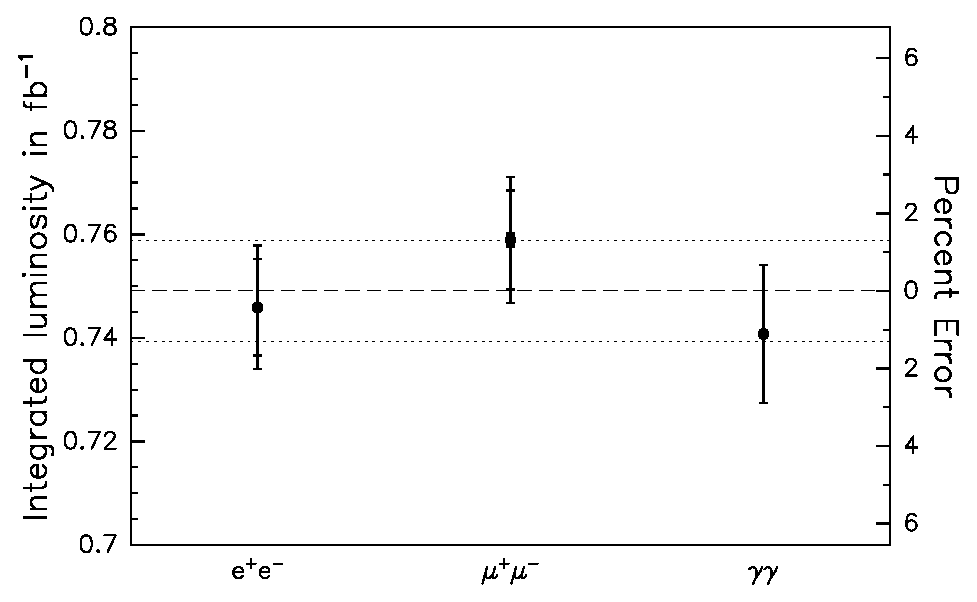
\includegraphics[width=0.65\linewidth]{../plenary_lumi}
\end{center}

\vspace{0.5 cm}
\begin{itemize}

  \item Blinded $\Gamma_{ee}$ by applying this normalization at the end

\end{itemize}

\end{slidemap1}

\begin{slidemap1}[technique & backgrounds & efficiency & luminosity & {\color{blue} stability} & fits & results & theory]

\vspace{0.5 cm}
\begin{center}
  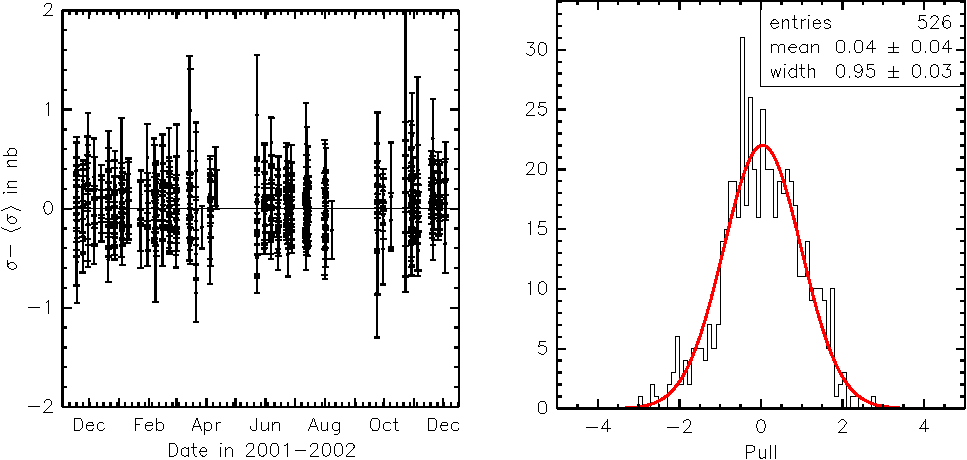
\includegraphics[width=0.95\linewidth]{../stability}
\end{center}

\vspace{0.5 cm}
\begin{itemizer}{0.75 cm}

  \item All off-resonance runs at a given energy reproduce the same
    cross-section

%%  \item Cross-section {\bf in}stability $\lesssim$ 0.03 nb

\end{itemizer}

\end{slidemap1}

\begin{slidemap1}[technique & backgrounds & efficiency & luminosity & {\color{blue} stability} & fits & results & theory]

\begin{tabular}{p{0.6\linewidth} p{0.38\linewidth}}
  \begin{minipage}{\linewidth}
    \begin{minipage}{0.9\linewidth}
      \begin{center}
	Beam energy reproducibility
      \end{center}

      \vspace{2 cm}
      \begin{itemizer}{2 cm}
	\item Each resonance was completely scanned once a week
        \item Measurements alternated above and below resonance peak
        \item A point of high slope was repeated in the scan
	\end{itemizer}
    \end{minipage}

  \end{minipage} &
  \begin{minipage}{\linewidth}
    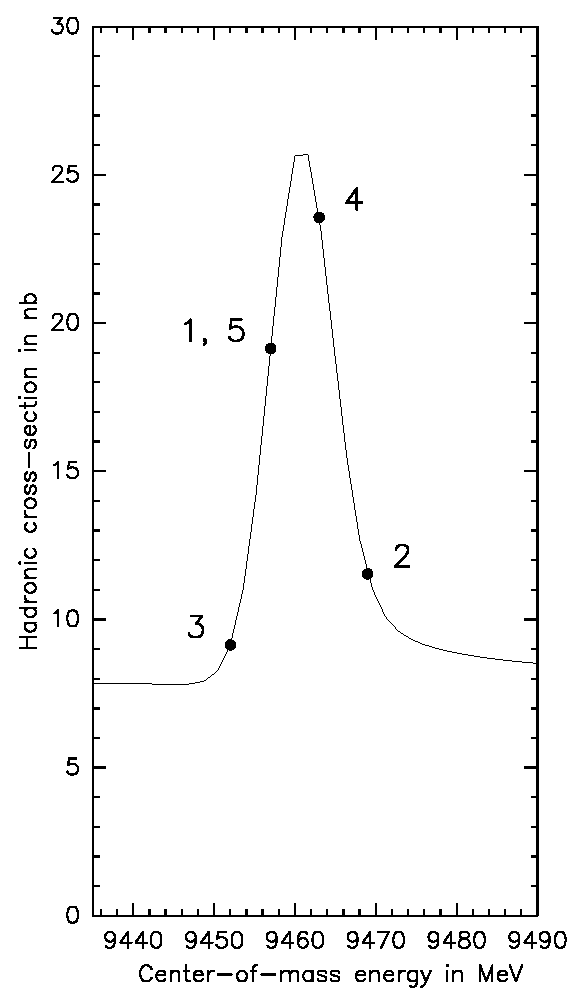
\includegraphics[width=\linewidth]{../plenary_fitorder}
  \end{minipage}
\end{tabular}

\end{slidemap1}

\begin{slidemap1}[technique & backgrounds & efficiency & luminosity & {\color{blue} stability} & fits & results & theory]

\vspace{0.5 cm}
\begin{itemizer}{0.5 cm}

  \item Repeated point $\longrightarrow$ beam energy reproducibility

  \item 29 pairs are scattered statistically

\end{itemizer}

\vspace{1 cm}
\begin{center}
  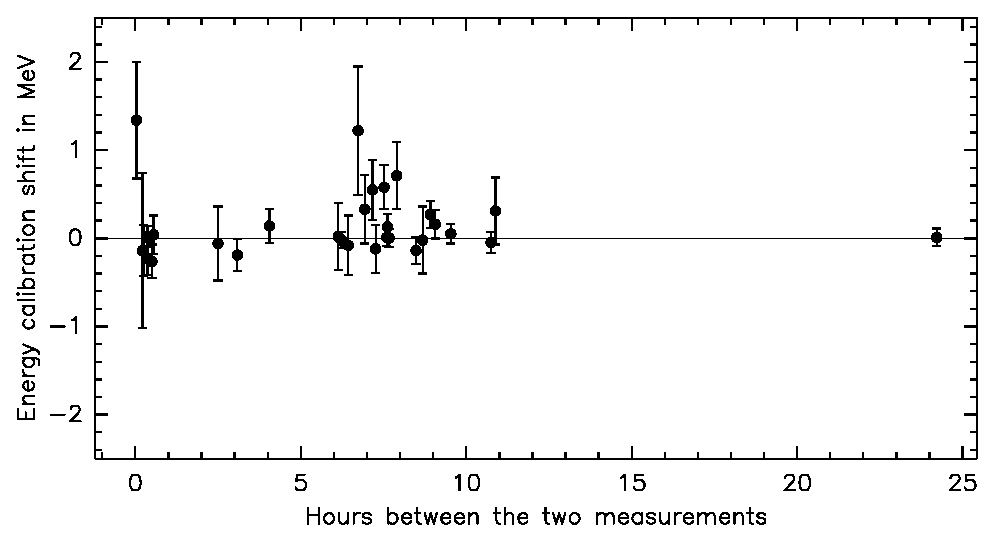
\includegraphics[width=0.7\linewidth]{../proceedings_miscal}
\end{center}

\vspace{1 cm}
\begin{itemize}

  \item Beam-energy reproducible at 0.07 MeV, $\Gamma_{ee}$ uncertainty $\lesssim$ 0.2\%

\end{itemize}

\end{slidemap1}

\begin{slidemap1}[technique & backgrounds & efficiency & luminosity & stability & {\color{blue} fits} & results & theory]

\begin{tabular}{p{0.6\linewidth} p{0.38\linewidth}}
  \begin{minipage}{\linewidth}
    {\bf Parameters:}

    \vspace{1 cm}
    \mbox{\hspace{1 cm}} \begin{minipage}{0.85\linewidth}
      \begin{enumerate}\setlength{\itemsep}{0.75 cm}
        \item Area without tail (MeV nb)

	  \hfill $\longrightarrow$ $\Gamma_{ee}$ (keV)
	  
        \item Beam energy spread (MeV)

        \item Background level (nb)
          \renewcommand{\labelenumi}{4--15.}

        \item $\Upsilon$ mass for each weekly scan (MeV)

      \end{enumerate}
    \end{minipage}

    \vspace{4 cm}
  \end{minipage} &
  \begin{minipage}{\linewidth}
    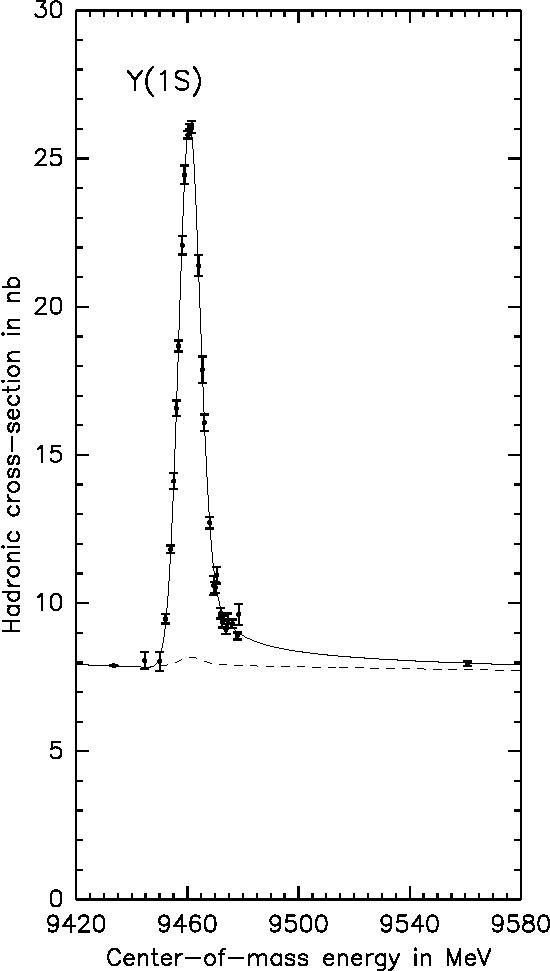
\includegraphics[width=\linewidth]{../individual_noinset_1s}
  \end{minipage}
\end{tabular}

\end{slidemap1}

\begin{slidemap1}[technique & backgrounds & efficiency & luminosity & stability & {\color{blue} fits} & results & theory]

\vspace{0.75 cm}
\begin{center}
  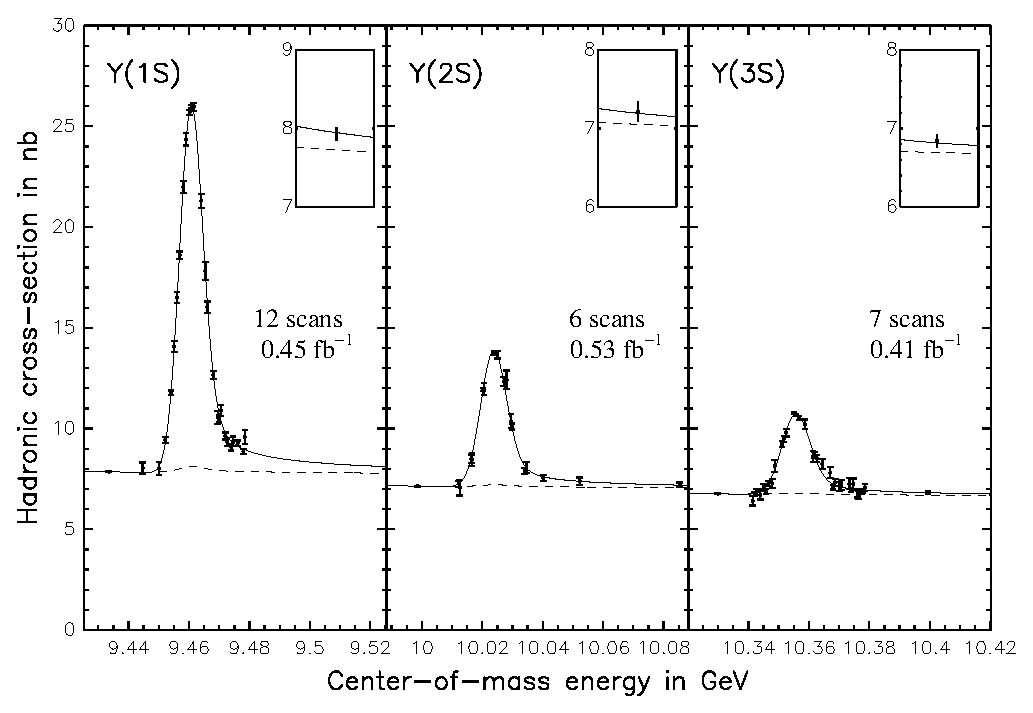
\includegraphics[width=0.93\linewidth]{../three_resonances_inset_squat2_nscans}
\end{center}
\vspace{-0.75 cm}

\end{slidemap1}

\begin{slidemap1}[technique & backgrounds & efficiency & luminosity & stability & {\color{blue} fits} & results & theory]

\begin{itemize}

  \item Best before CLEO-III

\end{itemize}

\vspace{1 cm}
\begin{center}
  \begin{tabular}{p{0.3\linewidth} p{0.3\linewidth} p{0.3\linewidth}}
    \begin{minipage}{\linewidth}
      \begin{center}
        Novosibirsk 1996
      \end{center}
    \end{minipage} &
    \begin{minipage}{\linewidth}
      \begin{center}
        \mbox{\hspace{0.3 cm}} ARGUS 1994
      \end{center}
    \end{minipage} &
    \begin{minipage}{\linewidth}
      \begin{center}
        CLEO-I 1984
      \end{center}
    \end{minipage}
  \end{tabular}
  \begin{tabular}{p{0.3\linewidth} p{0.3\linewidth} p{0.3\linewidth}}
    \begin{minipage}{\linewidth}
      \begin{center}
        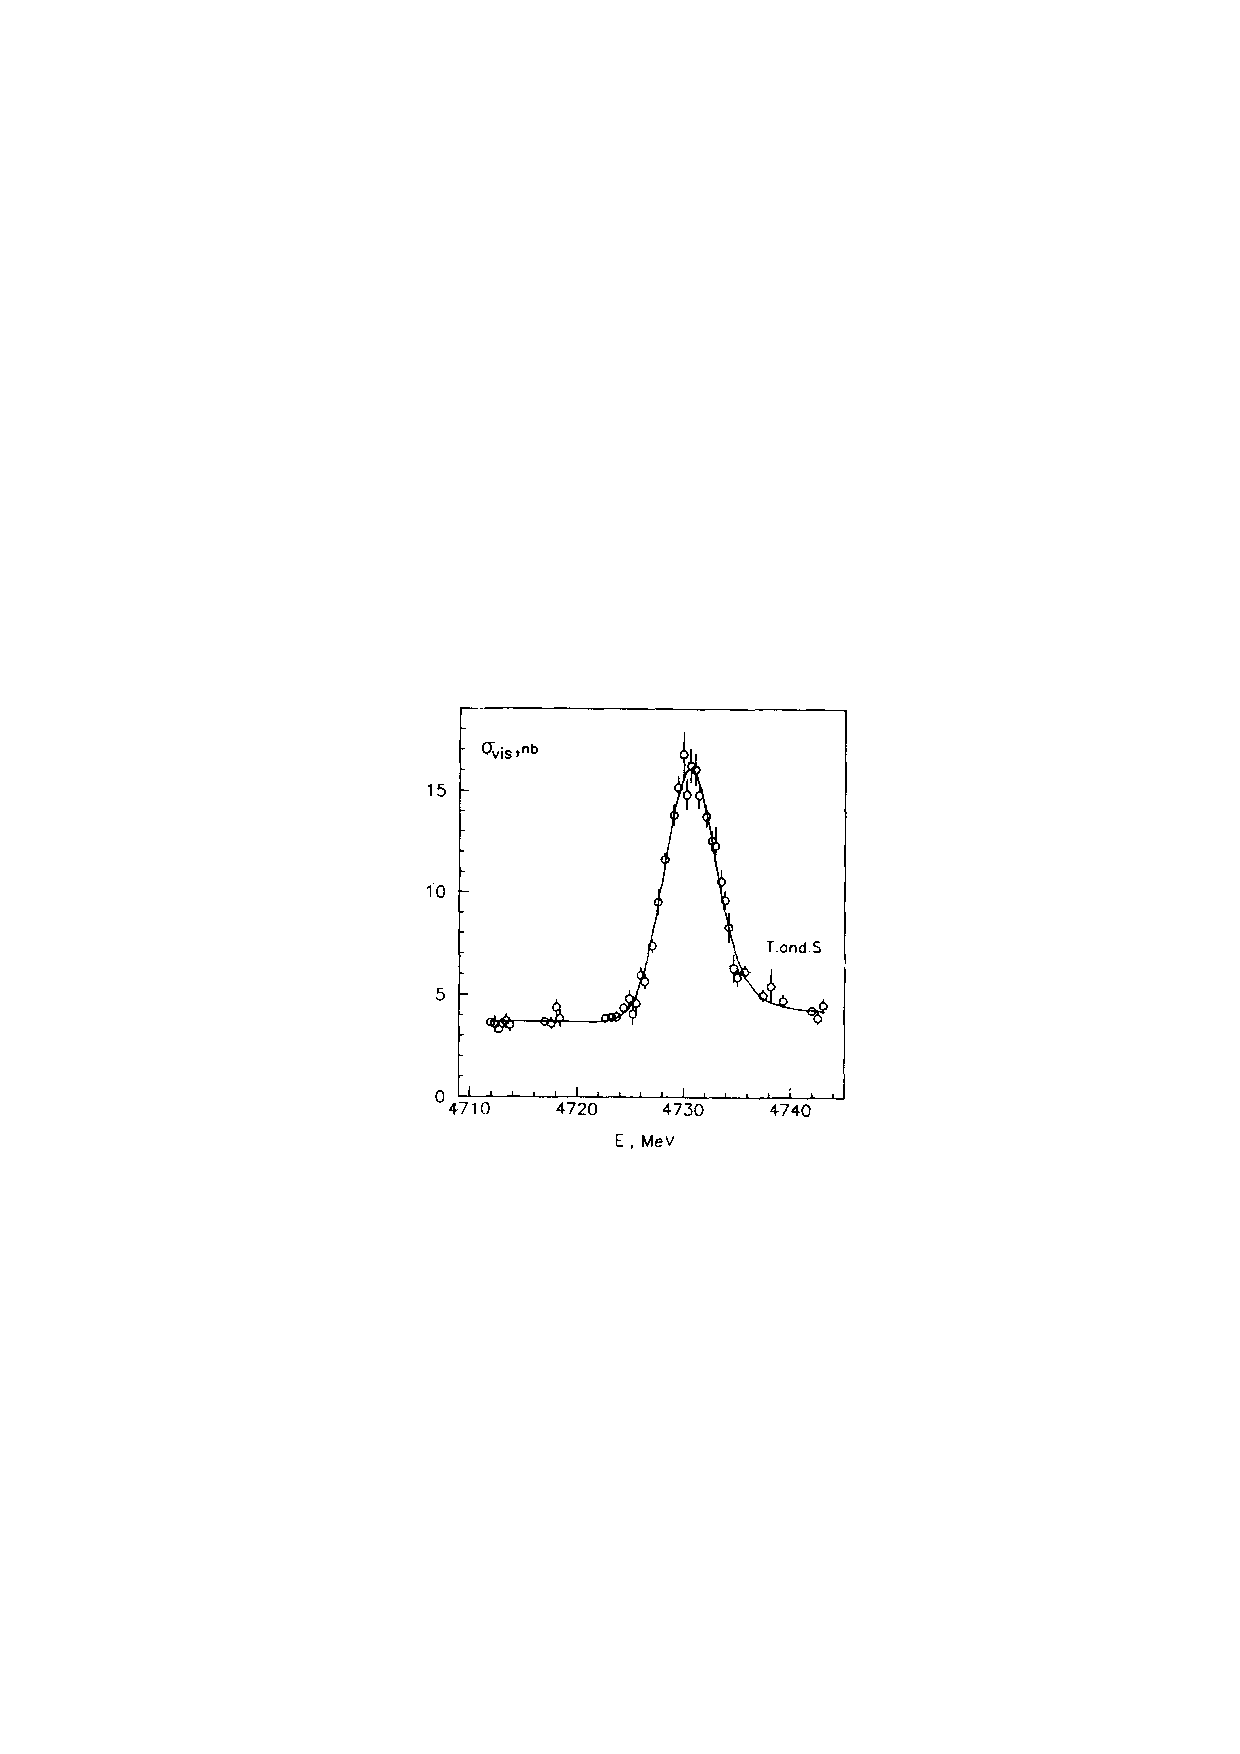
\includegraphics[width=\linewidth, height=\linewidth]{novo_y1s}
      \end{center}
    \end{minipage} &
    \begin{minipage}{\linewidth}
      \begin{center}
        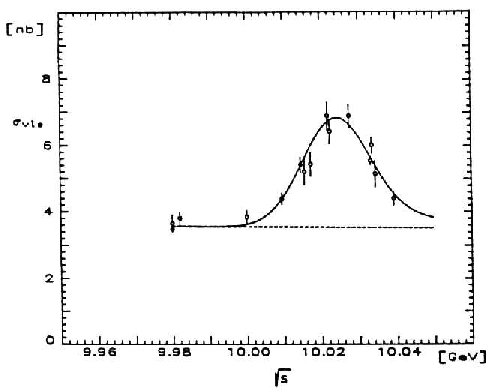
\includegraphics[width=\linewidth, height=\linewidth]{argus_y2s}
      \end{center}
    \end{minipage} &
    \begin{minipage}{\linewidth}
      \begin{center}
        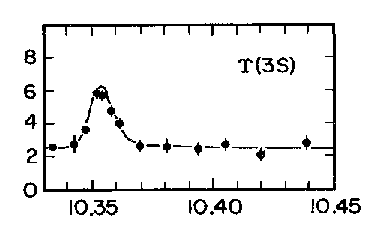
\includegraphics[width=\linewidth, height=\linewidth]{cleo1_y3s}
      \end{center}
    \end{minipage}
  \end{tabular}
  \begin{minipage}{\linewidth}
    \vspace{-6.4 cm}
    \begin{tabular}{p{0.3\linewidth} p{0.3\linewidth} p{0.3\linewidth}}
      \centering \LARGE $\Upsilon(1S)$ \hspace{1 cm} & \centering \LARGE $\Upsilon(2S)$ & 
    \end{tabular}
    \vspace{6.4 cm}
  \end{minipage}
  \begin{minipage}{\linewidth}
    \begin{tabular}{p{0.3\linewidth} p{0.3\linewidth} p{0.3\linewidth}}
      \begin{minipage}{\linewidth} \begin{center} \mbox{\hspace{1.3 cm}} 3.3\% \end{center} \end{minipage} & \begin{minipage}{\linewidth} \begin{center} \mbox{\hspace{2 cm}} 6.1\% \end{center} \end{minipage} & \begin{minipage}{\linewidth} \begin{center} \mbox{\hspace{1.7 cm}} 9.4\% \end{center} \end{minipage}
    \end{tabular}
  \end{minipage}
\end{center}

\end{slidemap1}

\begin{slidemap1}[technique & backgrounds & efficiency & luminosity & stability & {\color{blue} fits} & results & theory]

\vspace{0.75 cm}
\begin{center}
  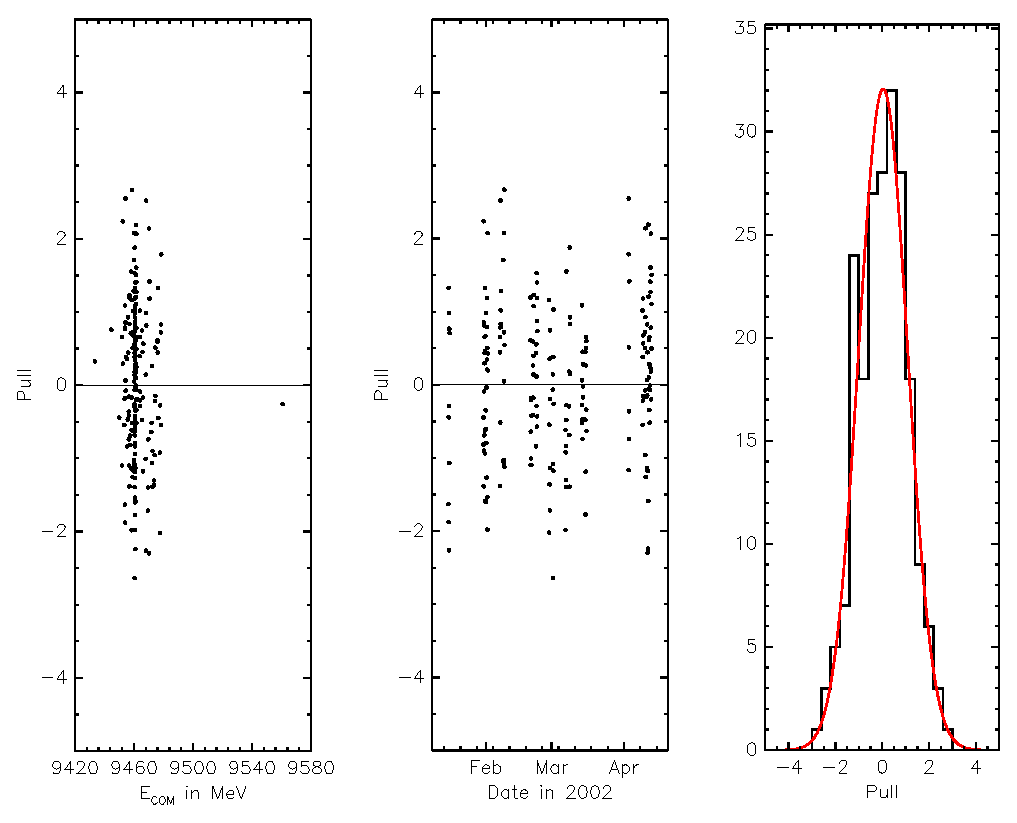
\includegraphics[width=0.74\linewidth]{../plenary_pulls1}
\end{center}
$\Upsilon(1S)$ Pull Distributions: $\chi^2/$ndf = 230/195 = 1.2, C.L. = 4\%
\vspace{-0.75 cm}

\end{slidemap1}

\begin{slidemap1}[technique & backgrounds & efficiency & luminosity & stability & {\color{blue} fits} & results & theory]

\vspace{0.75 cm}
\begin{center}
  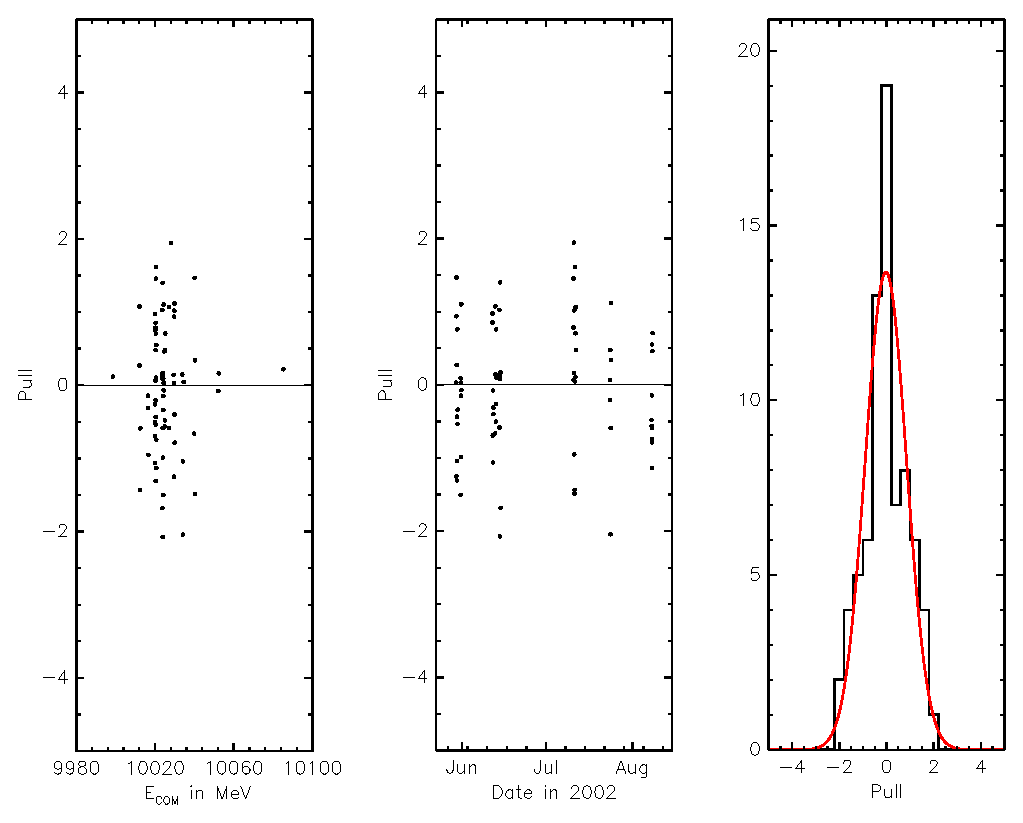
\includegraphics[width=0.74\linewidth]{../plenary_pulls2}
\end{center}
$\Upsilon(2S)$ Pull Distributions: $\chi^2/$ndf = 58/66 = 0.87, C.L. = 76\%
\vspace{-0.75 cm}

\end{slidemap1}

\begin{slidemap1}[technique & backgrounds & efficiency & luminosity & stability & {\color{blue} fits} & results & theory]

\vspace{0.75 cm}
\begin{center}
  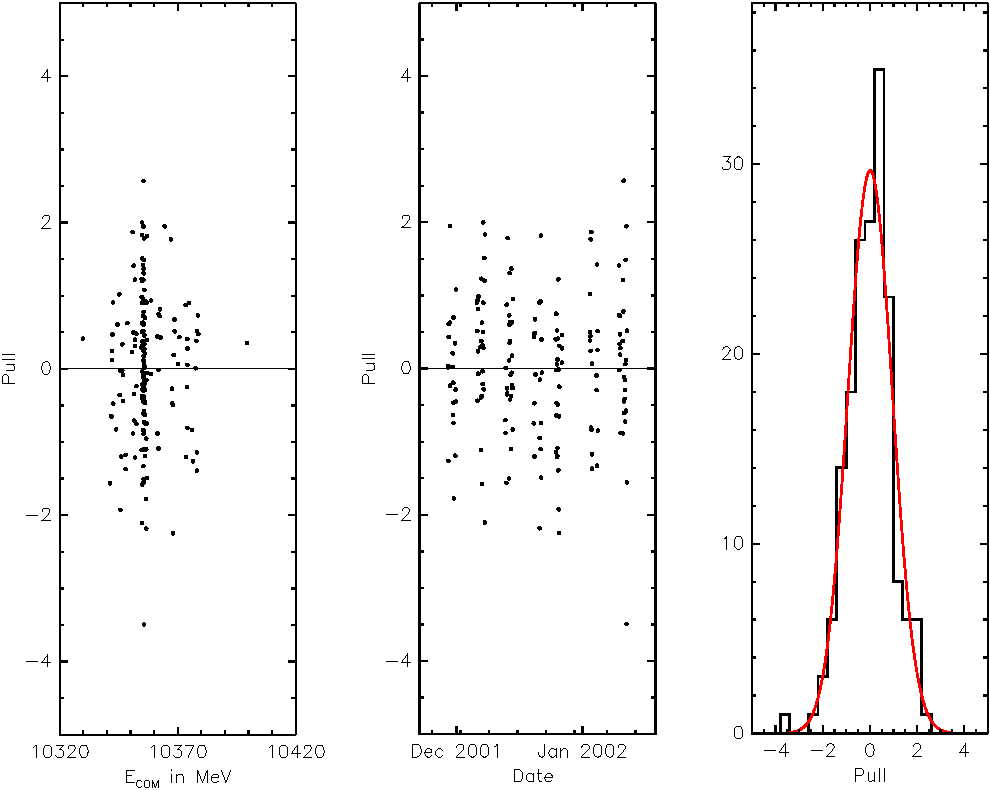
\includegraphics[width=0.74\linewidth]{../plenary_pulls3}
\end{center}
$\Upsilon(3S)$ Pull Distributions: $\chi^2/$ndf = 155/165 = 0.94, C.L. = 70\%
\vspace{-0.75 cm}

\end{slidemap1}

\begin{slidemap1}[technique & backgrounds & efficiency & luminosity & stability & fits & {\color{blue} results} & theory]

Summary of Uncertainties
\begin{center}
  \renewcommand{\arraystretch}{1.25}
  \begin{tabular}{l c c c}
    Contribution to $\Gamma_{ee}$ & \mbox{\hspace{0.75 cm}} $\Upsilon(1S)$ \mbox{\hspace{0.75 cm}} & \mbox{\hspace{0.75 cm}} $\Upsilon(2S)$ \mbox{\hspace{0.75 cm}} & \mbox{\hspace{0.75 cm}} $\Upsilon(3S)$ \mbox{\hspace{0.75 cm}} \\\hline
    Statistical$^*$               & {\color{red} 0.7\%}  & {\color{red} 1.6\%}  & {\color{red} 2.2\%} \\
    Correction for leptonic modes & 0.2\%  & 0.2\%  & 0.3\% \\
    Hadronic efficiency           & 0.5\%  & 0.6\%  & 0.7\% \\
    Overall luminosity scale      & {\color{red} 1.3\%}  & {\color{red} 1.3\%}  & {\color{red} 1.3\%} \\
    Cross-section measurement     & 0.1\%  & 0.1\%  & 0.1\% \\
    Beam-energy measurement       & 0.2\%  & 0.2\%  & 0.2\% \\
    Shape of the fit function     & 0.05\% & 0.06\% & 0.05\% \\\hline
    Total                         & {\color{red} 1.6\%}  & {\color{red} 2.2\%}  & {\color{red} 2.7\%} \\
  \end{tabular}
\end{center}

\mbox{ }$^*$\begin{minipage}{0.9\linewidth}

  \vspace{1 cm}
  Statistical uncertainty is dominated by run-by-run luminosity
  measurement ($\gamma\gamma$ counting)
\end{minipage}

\end{slidemap1}

\begin{slidemap1}[technique & backgrounds & efficiency & luminosity & stability & fits & {\color{blue} results} & theory]

\textcolor{red}{Preliminary Results}

\vfill

\vspace{-1 cm}
\begin{center}
  \renewcommand{\arraystretch}{1.5}
  \begin{tabular}{c c c}
    Quantity & Value & \mbox{\hspace{0.5 cm}} Uncertainty \mbox{\hspace{0.5 cm}} \\ \hline
    $\Gamma_{ee}(1S)$ & \mbox{\hspace{0.5 cm}} 1.336 $\pm$ 0.009 $\pm$ 0.019 keV \mbox{\hspace{0.5 cm}} & 1.6\% \\
    $\Gamma_{ee}(2S)$ & 0.616 $\pm$ 0.010 $\pm$ 0.009 keV & 2.2\% \\
    $\Gamma_{ee}(3S)$ & 0.425 $\pm$ 0.009 $\pm$ 0.006 keV & 2.7\% \\ \hline
    $\Gamma_{ee}(2S)$/$\Gamma_{ee}(1S)$ & 0.461 $\pm$ 0.008 $\pm$ 0.003 & 1.8\% \\
    $\Gamma_{ee}(3S)$/$\Gamma_{ee}(1S)$ & 0.318 $\pm$ 0.007 $\pm$ 0.002 & 2.4\% \\
    $\Gamma_{ee}(3S)$/$\Gamma_{ee}(2S)$ & 0.690 $\pm$ 0.019 $\pm$ 0.006 & 2.8\% \\
  \end{tabular}
\end{center}

\vfill
Presented at EPS, Lattice05, PANIC05

\end{slidemap1}

\begin{slidemap1}[technique & backgrounds & efficiency & luminosity & stability & fits & {\color{blue} results} & theory]

\vspace{0.25 cm}
\begin{center}
  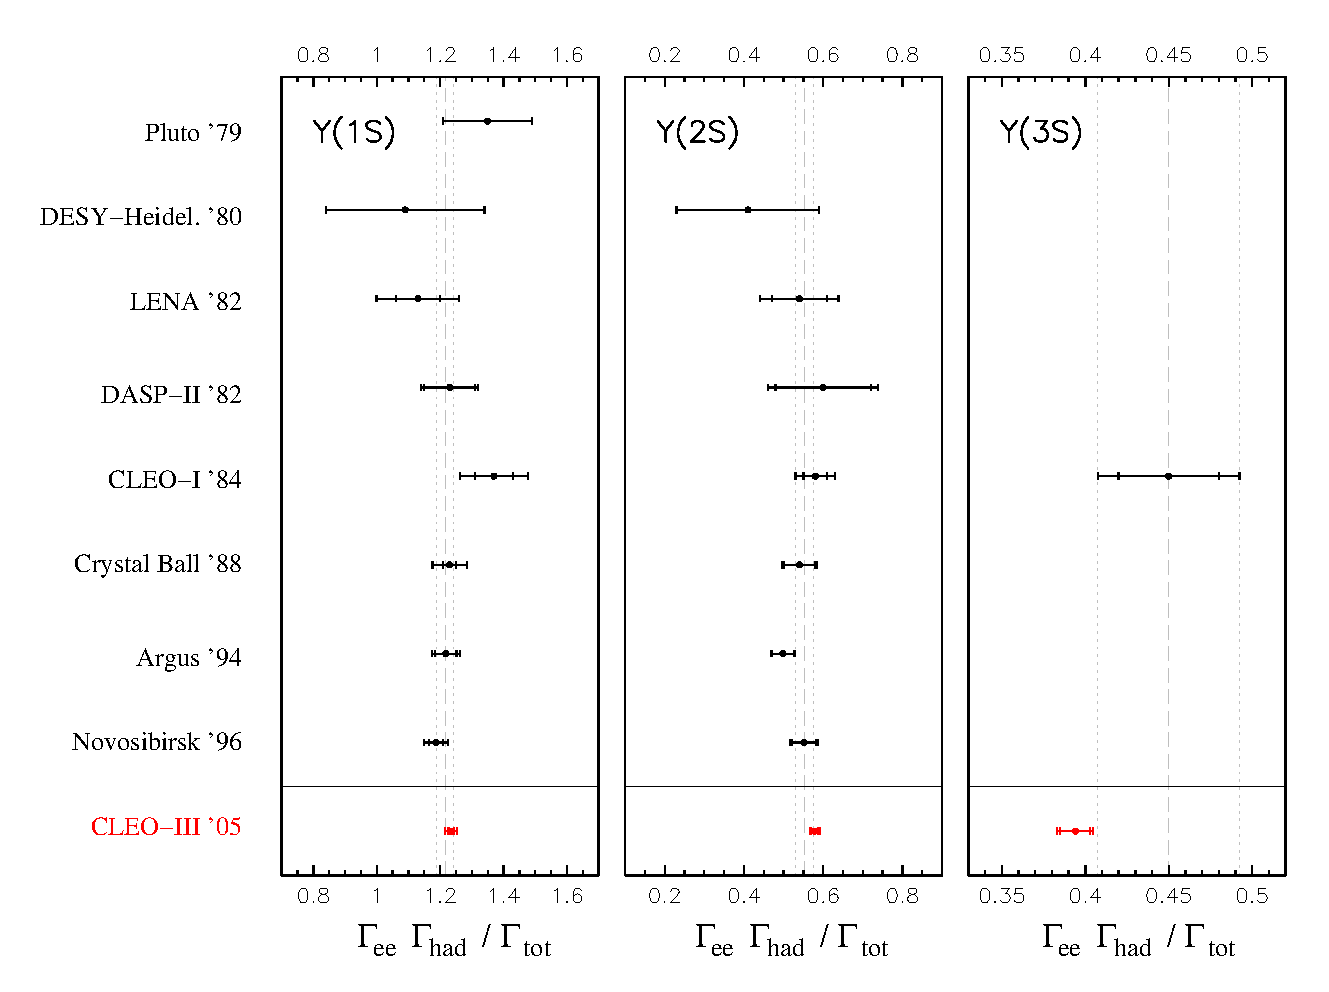
\includegraphics[width=0.95\linewidth, trim=0 0.5cm 0 1.8cm]{../pdgplots2}
\end{center}
\vspace{-1.25 cm}

\end{slidemap1}

\begin{slidemap1}[technique & backgrounds & efficiency & luminosity & stability & fits & {\color{blue} results} & theory]

\begin{center}
  \includegraphics[width=0.8\linewidth]{/home/mccann/antithesis/plots/panic05/prettied-zoomed_pdgplots2}
\end{center}

\end{slidemap1}

\begin{slidemap1}[technique & backgrounds & efficiency & luminosity & stability & fits & results & {\color{blue} theory}]

\begin{itemizer}{0.5 cm}

  \item LQCD result not yet complete

  \item But we can compare {\it ratio} of $\Gamma_{ee}(2S)/\Gamma_{ee}(1S)$ (missing factor cancels)

\end{itemizer}

\vfill

\begin{center}
  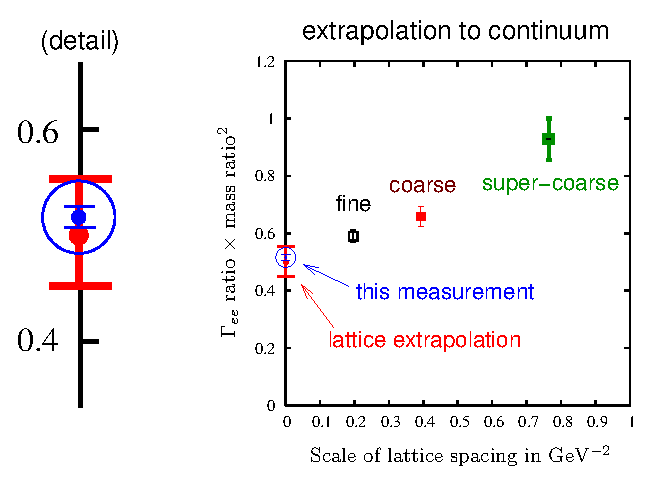
\includegraphics[width=0.75\linewidth]{dependence}
  %% (hep-lat:0507013, 13 July 2005)
\end{center}

\end{slidemap1}

\begin{slidemap1}[technique & backgrounds & efficiency & luminosity & stability & fits & results & {\color{blue} theory}]

\begin{itemizer}{0.5 cm}

  \item Why does the lattice result have 10\% uncertainty?

    \vspace{0.4 cm}
\[ \Gamma_{ee} = \frac{16\pi\alpha^2e_b^2}{6{M_\Upsilon}^2} \underbrace{\mathhi \langle \Upsilon | J_\nu | 0 \rangle^2 \mathhi}_{\mbox{\hspace{-2 cm} wavefunction at origin \hspace{-2 cm}}} {Z_{match}}^2 \]

  \item Wavefunction at origin is particularly sensitive to discretization

\begin{center}
  \begin{tabular}{p{5 cm} p{1 cm} p{5 cm}}
    \mbox{\begin{minipage}{\linewidth} 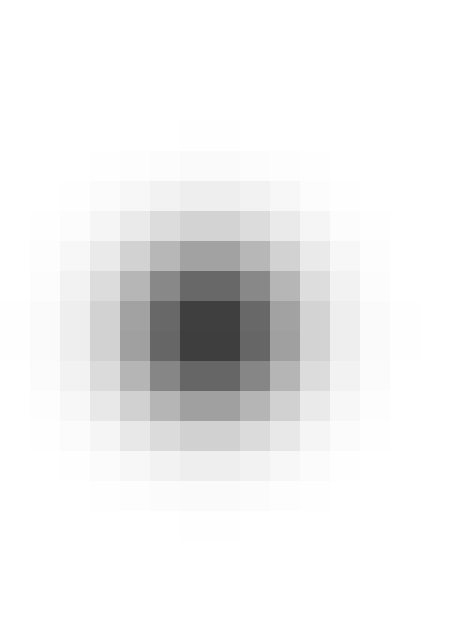
\includegraphics[width=\linewidth, trim=0 2.2cm 0 2.2cm, clip=true]{../fuzzyloose-digital} \end{minipage}} & \mbox{\begin{minipage}{\linewidth} vs \end{minipage}} & \mbox{\begin{minipage}{\linewidth} 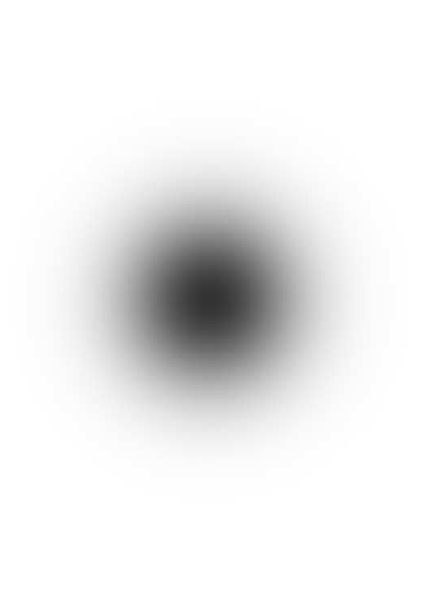
\includegraphics[width=\linewidth, trim=0 2.2cm 0 2.2cm, clip=true]{../fuzzyloose} \end{minipage}}
  \end{tabular}
\end{center}

  \vspace{0.25 cm}
  \item Missing factor ($Z_{match}$) corrects for discretization

  \item Predicted precision: few percent on ratios, 10\% on absolute values

\end{itemizer}

\end{slidemap1}

\begin{slide}[Conclusion for $\Gamma_{ee}(\Upsilon)$]

\begin{center}
  \begin{tabular}{p{0.4\linewidth} p{0.13\linewidth}}
    \begin{minipage}{\linewidth}
      \includegraphics[width=\linewidth]{new_ratio_plot}
    \end{minipage} &
  \end{tabular}
\end{center}

\vfill

\begin{itemizer}{0.75 cm}

  \item Final experimental results (not yet released):

    \begin{center}
      \renewcommand{\arraystretch}{1.25}
      \begin{tabular}{c c c}
	$\Gamma_{ee}(1S)$ & $\Gamma_{ee}(2S)$ & $\Gamma_{ee}(3S)$ \\
	$\pm$1.5\% & $\pm$1.9\% & $\pm$1.8\% \\
	$\Gamma_{ee}(2S)/\Gamma_{ee}(1S)$ & \mbox{\hspace{0.5 cm}} $\Gamma_{ee}(3S)/\Gamma_{ee}(1S)$ \mbox{\hspace{0.5 cm}} & $\Gamma_{ee}(3S)/\Gamma_{ee}(2S)$ \\
	$\pm$1.4\% & $\pm$1.2\% & $\pm$1.7\%
      \end{tabular}
    \end{center}

  \item Final theory results will be few percent in ratios

\end{itemizer}

\end{slide}

\begin{slide}

\vfill
\begin{center}
  \fbox{\includegraphics[height=1.5 cm]{title_fD}}
\end{center}

\vfill
\begin{itemizer}{1 cm}

  \item CLEO-c, the next generation of CLEO

  \item Very different kind of analysis: discovery, statistics-limited

\end{itemizer}

\vfill

\end{slide}

\begin{slidemap2}[{\color{blue} introduction} & event selection & results]

\vspace{0.5 cm}
\begin{itemizer}{0.5 cm}

  \item CLEO-c: new inner tracker, charm energies

  \item 281 pb\inv\ at $\psi(3770)$: 3 million $D\bar{D}$

\end{itemizer}

\vfill
\begin{center}
  \includegraphics[width=0.7\linewidth]{../cleoc_2}
\end{center}

\end{slidemap2}

\begin{slidemap2}[{\color{blue} introduction} & event selection & results]

\begin{center}
  \begin{tabular}{p{0.5\linewidth} p{0.45\linewidth}}
    \begin{minipage}{\linewidth}
      \includegraphics[width=\linewidth]{../dmunu_event}
    \end{minipage} &
    \begin{minipage}{\linewidth}
      \begin{itemizer}{0.5 cm}

	\item Fully reconstruct $D^-$ decay, search for $D^+ \to \mu^+ \nu$

	  \vspace{0.25 cm}
	  \renewcommand{\arraystretch}{1.25}
	  \begin{center}
            \begin{tabular}{l}
  	      $D^-$ Tag Modes \\\hline\hline
  	      $K^+\,\pi^-\,\pi^-$ \\
  	      $K^+\,\pi^-\,\pi^-\,\pi^0$ \\
  	      $K_S\,\pi^-$ \\
  	      $K_S\,\pi^-\,\pi^-\,\pi^+$ \\
  	      $K_S\,\pi^-\,\pi^0$ \\
  	      $K^+\,K^-\,\pi^-$ \\
            \end{tabular}
	  \end{center}

      \end{itemizer}
    \end{minipage}
  \end{tabular}
\end{center}

\end{slidemap2}

\begin{slidemap2}[introduction & {\color{blue} event selection} & results]

\vspace{-2 cm}
\begin{center}
  \begin{tabular}{p{0.6\linewidth} p{0.35\linewidth}}
    \begin{minipage}{\linewidth}
      \begin{itemize}

	\item RICH detector for $\mu/K$, $\pi/K$ separation

      \end{itemize}
    \end{minipage} &
    \begin{minipage}{\linewidth}
      \includegraphics[width=\linewidth]{../rich_kpisep2}
    \end{minipage}
  \end{tabular}

  \begin{tabular}{p{0.45\linewidth} p{0.5\linewidth}}
    \begin{minipage}{\linewidth}
      \begin{itemize}

	\item Mass of reconstructed $D^-$

      \end{itemize}
    \end{minipage} &
    \begin{minipage}{\linewidth}
      \includegraphics[width=\linewidth, clip=true]{../dmunu_mbc}
    \end{minipage}
  \end{tabular}
\end{center}

\end{slidemap2}

\begin{slidemap2}[introduction & {\color{blue} event selection} & results]

\begin{center}
  \begin{tabular}{p{0.7\linewidth} c p{0.25\linewidth}}
    \begin{minipage}{\linewidth}
      \begin{center}
	\includegraphics[width=\linewidth, viewport=0 28 365 350, clip=true]{../dmunu_mm}
	\mbox{\hspace{1.5 cm}} $\nu$ missing mass$^{\mathsf{2}}$ in GeV$^{\mathsf{2}}$
      \end{center}
    \end{minipage} & &
    \begin{minipage}{\linewidth}
      \renewcommand{\arraystretch}{1.5}
      \begin{tabular}{r}
	50 events \\
	$-$ 2.8 background \\\hline
	47.2 $\pm$ 7.1 $^{\mathsf{+0.3}}_{\mathsf{-0.8}}$
      \end{tabular}
    \end{minipage}
  \end{tabular}
\end{center}

\end{slidemap2}

\begin{slidemap2}[introduction & event selection & {\color{blue} results}]

\vspace{0.25 cm}
\begin{itemizer}{0.5 cm}

  \item $\mathcal{B}(D^+ \to \mu^+\nu)$ = (4.40 $\pm$ 0.66 $^{{\mathsf{+0.09}}}_{{\mathsf{-0.12}}}$) $\times$ 10$^{{\mathsf{-4}}}$ \hfill (15\% statistical)

  \item $f_{D^+}$ = (222.6 $\pm$ 16.7 $^{{\mathsf{+2.8}}}_{{\mathsf{-3.4}}}$) MeV \hfill (7.5\% statistical)

\end{itemizer}

\vspace{0.25 cm}
\begin{center}
  \includegraphics[width=0.47\linewidth]{dmunu_comparison3}
\end{center}
\vspace{-1 cm}

\end{slidemap2}

\begin{slide}[Conclusion for $f_D$]

\begin{center}
  \begin{tabular}{p{0.4\linewidth} p{0.13\linewidth}}
    \begin{minipage}{\linewidth}
      \includegraphics[width=\linewidth]{new_ratio_plot2}
    \end{minipage} &
  \end{tabular}
\end{center}

\vfill

\begin{itemizer}{1 cm}

  \item $\frac{\mbox{Projected 750 fb\inv\ by April 2008}}{\mbox{281 fb\inv\ so far}} \to$ 5\% uncertainty in $f_D$

  \item CLEO-c found a 0.9 nb $D_s{D_s}^*$ resonance at 4.17 GeV \\
    \mbox{ } \hfill $\to$ 15\% uncertainty in $f_{D_s}$ by 2008

\end{itemizer}

\end{slide}

\begin{slide}[Not just tests of LQCD]

\begin{itemizer}{0.5 cm}

  \item LQCD uncertainties cancel in ratios

  \item Project CLEO-c measurements into $B$ sector

\[ f_B = \left(\mathhie f_D \mathhie\right)_{\mbox{experiment}} \times \left(\frac{f_B}{f_D}\right)_{\mbox{LQCD}} \]

and

\[ f_{B_s}/f_B = \left(\mathhie f_{D_s}/f_D \mathhie\right)_{\mbox{experiment}} \times \left(\frac{f_{B_s}/f_B}{f_{D_s}/f_D}\right)_{\mbox{LQCD}} \]

\end{itemizer}

\begin{minipage}{0.48\linewidth}
  \begin{itemize}
  \item Applicable to two CKM bands
  \end{itemize}
\end{minipage} \hfill \begin{minipage}{0.4\linewidth}
  \includegraphics[width=\linewidth]{../ckm04}
\end{minipage}

\end{slide}

\begin{slide}[Related and interesting]

\vfill
\begin{center}
  \fbox{\begin{minipage}{19.5 cm}
      \begin{center}
	\includegraphics[height=1.5 cm]{title_Geepsi_again}
      \end{center}
  \end{minipage}}
\end{center}

\vfill
\begin{itemizer}{1 cm}

  \item $c\bar{c}$ version of $\Gamma_{ee}(\Upsilon)$

  \item New method: not a scan, but $e^+e^- \to \gamma \psi(2S)$ where $\sqrt{s}$ $\gg$ $M_{\psi(2S)}$

    \begin{itemizer}{0.75 cm}

      \item Cross-section on a resonance depends on beam energy spread

%% 	(wide beam $\Rightarrow$ low cross-section)

      \item Cross-section far above depends only on coupling to $e^+e^-$

    \end{itemizer}

  \item $\Gamma(J/\psi \to e^+e^-)$ also in progress

  \item BaBar is measuring all the $c\bar{c}$ and $b\bar{b}$ resonances this way!

\end{itemizer}

\vfill

\end{slide}

\begin{slide}

\begin{itemize}

  \item Look for $\psi(2S)$ in specific final states, such as $\pi^+\pi^- J/\psi$

\end{itemize}

\vfill

\begin{center}
  \includegraphics[width=0.8\linewidth]{psi_gamee2}
\end{center}

\vfill

\begin{itemizer}{0.5 cm}

  \item Limited by branching fraction measurements, which CLEO-c is improving

  \item $\Gamma_{ee}(\psi(2S))$ = 2.13 $\pm$ 0.03 $\pm$ 0.08 keV

\end{itemizer}

\end{slide}

\begin{slide}

\begin{itemize}

  \item This is another relevant test of LQCD: try all the flavor combinations!

\end{itemize}

\vfill

\begin{center}
  \renewcommand{\arraystretch}{2}
  \begin{tabular}{c c c c}
    & heavy-heavy & \mbox{\hspace{1 cm}} & heavy-light \\
    bottom \mbox{\hspace{1 cm}} & $\Gamma_{ee}(\Upsilon)$ & & $f_B$ \\
    & & & \\
    charm \mbox{\hspace{1 cm}} & $\Gamma_{ee}(\psi)$ & & $f_D$ \\
  \end{tabular}
\end{center}

\vfill
\begin{itemizer}{1 cm}

  \item LQCD can and will calculate $\Gamma_{ee}(\psi)$

  \item For $\Upsilon$, discretization is more significant

  \item For $\psi$, relativistic corrections are more significant

\end{itemizer}

\vspace{1 cm}

\end{slide}

\begin{slide}[Semileptonic form factors]

\begin{minipage}{0.52\linewidth}
  \begin{itemizer}{1 cm}

  \item $|V_{ub}|$ limited by form factor $f(q^2)$

  \item Much the same story as $f_B$:

    \vspace{0.25 cm}
    Can be calculated by LQCD and \mbox{extrapolated} from $D$ measurements

  \end{itemizer}
\end{minipage} \hfill \begin{minipage}{0.4\linewidth}
  \includegraphics[width=\linewidth]{../ckm04}
\end{minipage}

\begin{itemizer}{1 cm}

  \item $D$ measurements near threshold are much easier:

    less cross-feed, better $q^2$ resolution

\end{itemizer}

\begin{tabular}{p{0.47\linewidth} p{0.47\linewidth}}
  \begin{minipage}{\linewidth}
    \begin{center}
      CLEO-III (below $B\bar{B}$)
    \end{center}
  \end{minipage} & 
  \begin{minipage}{\linewidth}
    \begin{center}
      CLEO-c (at $D\bar{D}$ threshold)
    \end{center}
  \end{minipage} \\
  \begin{minipage}{\linewidth}
    \begin{center} \includegraphics[width=0.6\linewidth]{semilep_lauren3} \end{center}
  \end{minipage} &
  \begin{minipage}{\linewidth}
    \vspace{0.5 cm}

    \begin{center} \includegraphics[width=0.6\linewidth]{semilep_feng3} \end{center}
  \end{minipage} \\
  \begin{minipage}{\linewidth}
    \begin{center}
      \LARGE $D^0 \to {\pi^-} e^+ \nu$
    \end{center}
  \end{minipage} & 
  \begin{minipage}{\linewidth}
    \begin{center}
      \LARGE $D^0 \to {\pi^-} e^+ \nu$
    \end{center}
  \end{minipage}
\end{tabular}

\end{slide}

\begin{slide}[Conclusions]

\begin{minipage}{0.55\linewidth}
  \begin{itemizer}{0.75 cm}

    \item Two new points of contact between LQCD and experiment

    \item LQCD $\Gamma_{ee}(\Upsilon)$ result $\to$ few percent

    \item $f_D$ and $f_{D_s}$ $\to$ 5\% and 15\%

  \end{itemizer}
\end{minipage} \hfill \begin{minipage}{0.4\linewidth}
  \includegraphics[width=\linewidth]{new_ratio_plot2}
\end{minipage}

\vspace{0.5 cm}

\begin{itemizer}{0.75 cm}

  \item $\Gamma_{ee}(\psi)$ probes differences in treatment of charm and bottom quarks

  \item This is only part of the program: similar studies are being
  made of semileptonic form factors

\end{itemizer}

\end{slide}

\begin{slide}

\begin{itemizer}{1 cm}

  \item Tests of Lattice QCD useful are for weak physics applications

  \item But understanding the strong force quantitatively is interesting in itself

  \item Wouldn't it be nice to understand how the proton works?

\end{itemizer}

\vfill

\begin{center}
  \includegraphics[width=0.6\linewidth]{../qcd_proton}
\end{center}

\end{slide}

\end{document}
